Kiểm thử phần mềm là một bước quan trọng trong quy trình phát triển phần mềm, đảm bảo sản phẩm đáp ứng đầy đủ, chính xác những yêu cầu của khách hàng, giúp nhà phát triển phát hiện ra các lỗi tiềm ẩn, giảm thiểu các rủi ro và chi phí phát sinh trong quá trình bảo dưỡng và nâng cấp phần mềm trong tương lai.

Hệ thống website phòng Tổ chức-Hành chính được sử dụng trong việc quản lý thông tin, nghiệp vụ của cán bộ nhân viên nhà trường, vì vậy hệ thống phải đảm bảo được tính bảo mật, chính xác trong các tác vụ, tránh các lỗi gây ảnh hưởng, gián đoạn công việc của phòng Tổ chức-Hành chính và cán bộ nhân viên nhà trường. Vì vậy việc kiểm thử là vô cùng quan trọng và cần thiết trong quá trình xây dựng hệ thống.

Các công nghệ sử dụng trong kiểm thử thử hệ thống:
\begin{center}
  \captionsetup{type=figure}
  
\includegraphics[width=10cm]{img/mocha_chai.png}
  \captionof{figure}{Mocha framework và Chai assertion library}
\end{center}

Mocha là một Javascript framework kiểm thử chạy trên Node.js và trình duyệt, giúp cho việc kiểm tra bất đồng bộ một cách đơn giản. Mocha được đánh giá là một framework kiểm thử đơn giản, linh hoạt và chạy ổn định. Hiện nay, Mocha được nhiều công ty lớn sử dụng trong kiểm thử hệ thống.

Chai là một thư viện assertion với nhiều tuỳ chọn cho phép kiểm tra đối tượng như "should", "expect" và "assert". Trong hệ thống Tổ chức-Hành chính, nhóm nhận thấy có nhiều API có phương thức GET trả về dữ liệu dưới dạng JSON nên nhóm sử dụng Chai để thực hiện HTTP request và kiểm tra các giá trị trả về.

Nhận thấy sự đơn giản và phù hợp của Mocha framework và Chai assertion library, nhóm đã xây dựng hệ thống kiểm thử với 2 công nghệ trên để đảm bảo hệ thống hoạt động một cách tốt nhất khi đưa vào thực tế.

\section{Kiểm thử đơn vị (Unit Test)}
Kiểm thử đơn vị là một loại kiểm thử phần mềm, trong đó các thành phần đơn vị như method, class, function sẽ được kiểm thử. Kiểm thử đơn vị nhằm kiểm tra các tính năng riêng lẻ hoạt động đúng hay không. Ở phần này, nhóm kiểm thử các hàm xử lý thời gian, chuỗi, kiểm tra email,...
\begin{center}
  \captionsetup{type=figure}
  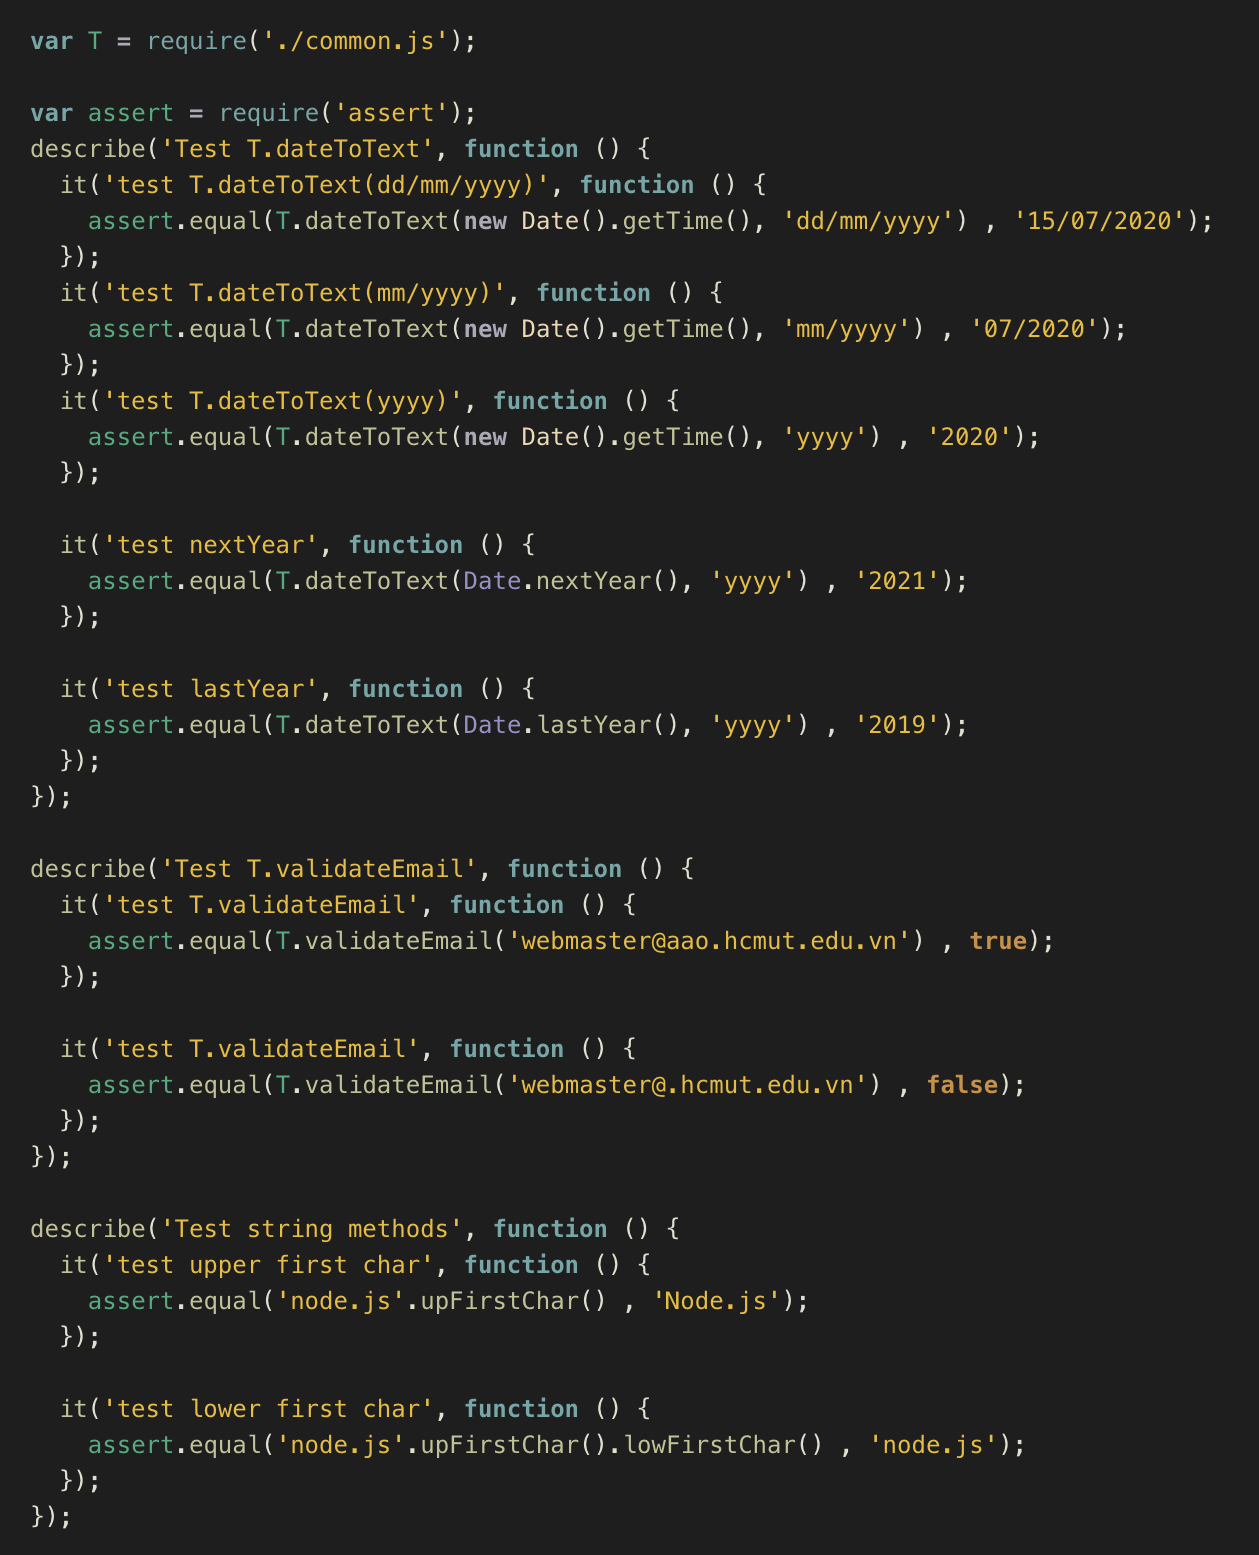
\includegraphics[width=15cm]{img/unitTestCode.png}
  \captionof{figure}{Đoạn code kiểm thử các hàm xử lý thời gian, chuỗi, kiểm tra email}
\end{center}
\newpage
Kết quả: 

\begin{center}
  \captionsetup{type=figure}
  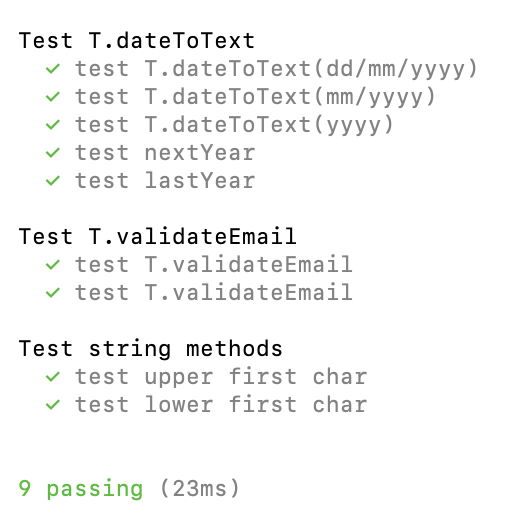
\includegraphics[width=7cm]{img/unitTestSolution.png}
  \captionof{figure}{Kết quả kiểm thử đơn vị}
\end{center}
\section{Kiểm thử tích hợp (Integration Test)}
Kiểm thử tích hợp là một giai đoạn trong kiểm thử phần mềm xảy ra sau khi kiểm thử đơn vị. Mục đích của kiểm thử tích hợp nhằm kiểm tra sự giao tiếp giữa các module, nhằm đảm bảo tính hợp nhất của hệ thống.
Nhóm đã sử dụng Mocha framework và Chai library để kiểm thử các API giao tiếp giữa tầng View và Controller.
\begin{center}
  \captionsetup{type=figure}
  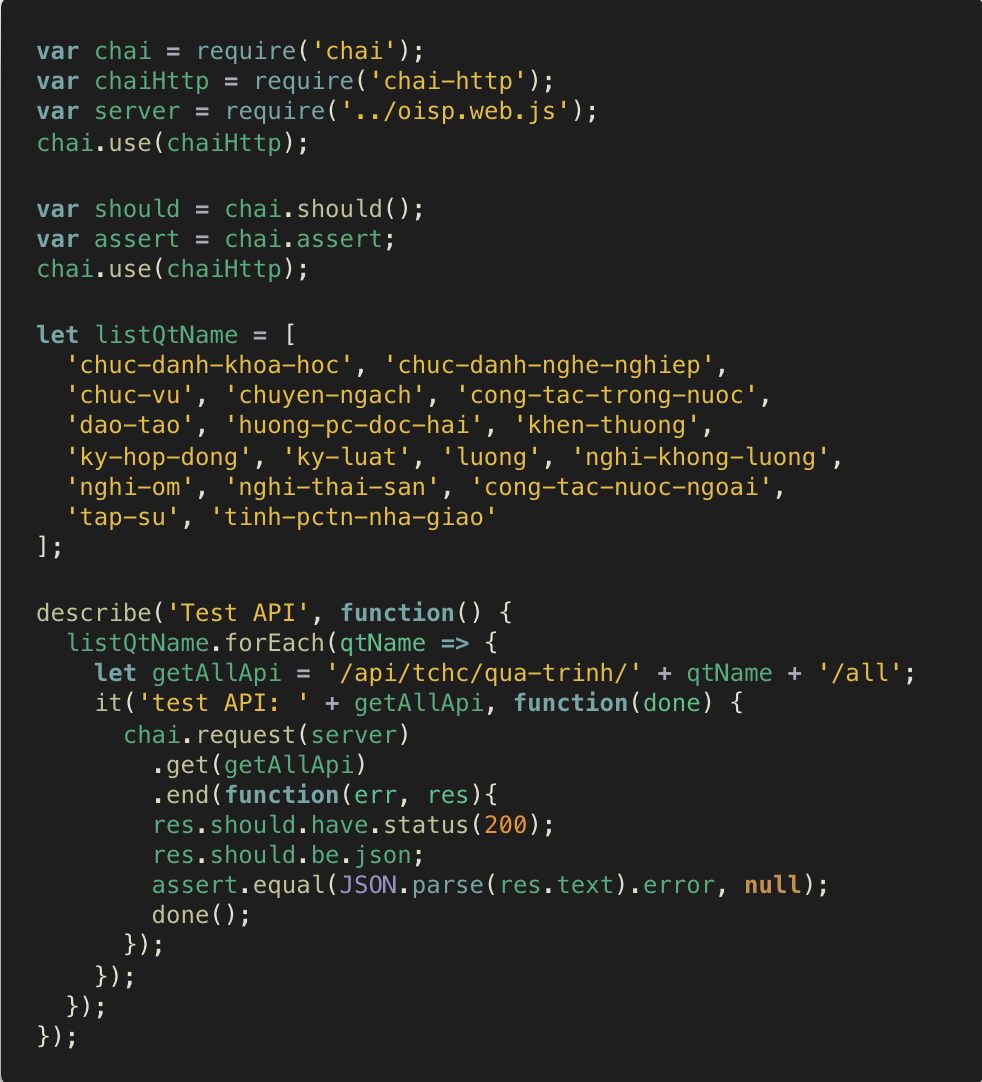
\includegraphics[width=15cm]{img/integrationTestCode.png}
  \captionof{figure}{Đoạn code kiểm thử các API giao tiếp giữa tầng View và Controller}
\end{center}
\newpage
Kết quả:
\begin{center}
  \captionsetup{type=figure}
  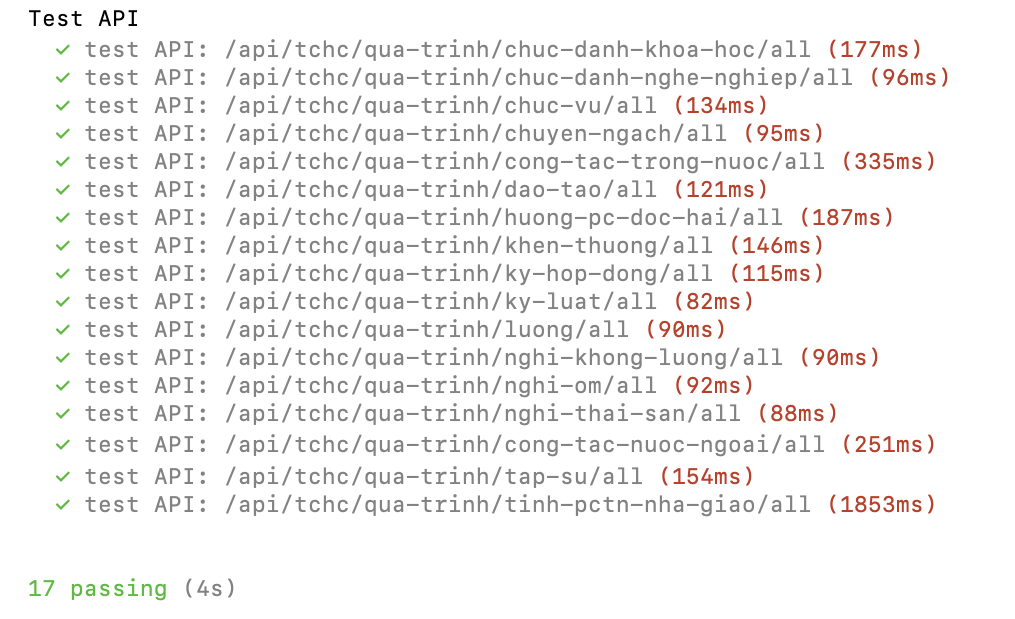
\includegraphics[width=15cm]{img/integrationTestSolution.png}
  \captionof{figure}{Kết quả kiểm thử tích hợp}
\end{center}
\section{Kiểm thử hệ thống (System Test)}
Kiểm thử hệ thống là giai đoạn kiểm thử nhằm kiểm tra sự hoàn chỉnh và tích hợp đầy đủ của hệ thống. Kiểm thử hệ thống là phương pháp kiểm thử hộp đen vì chỉ kiểm thử thông qua giao diện bên ngoài. Phương pháp kiểm thử này nhằm mục đích tìm ra các lỗi như:
\begin{itemize}
    \item Chức năng thiếu hoặc không chính xác.
    \item Lỗi truy cập cơ sở dữ liệu từ bên ngoài.
    \item Lỗi giao diện.
    \item Lỗi hiệu suất.
\end{itemize}
Trong quá trình phát triển hệ thống, nhóm tiến hành kiểm thử các chức năng của hệ thống như xem, tạo mới, sửa đổi, xoá thông tin với nhiều vai trò khác nhau như cán bộ phòng Tổ chức-Hành chính và người dùng hệ thống.
\subsection{Quy trình kiểm thử quản lý quá trình công tác trong nước với vai trò cán bộ phòng Tổ chức-Hành chính}
Tạo mới quá trình -> Chỉnh sửa quá trình -> Xoá quá trình

Danh sách quá trình công tác trong nước ban đầu.
\begin{center}
  \captionsetup{type=figure}
  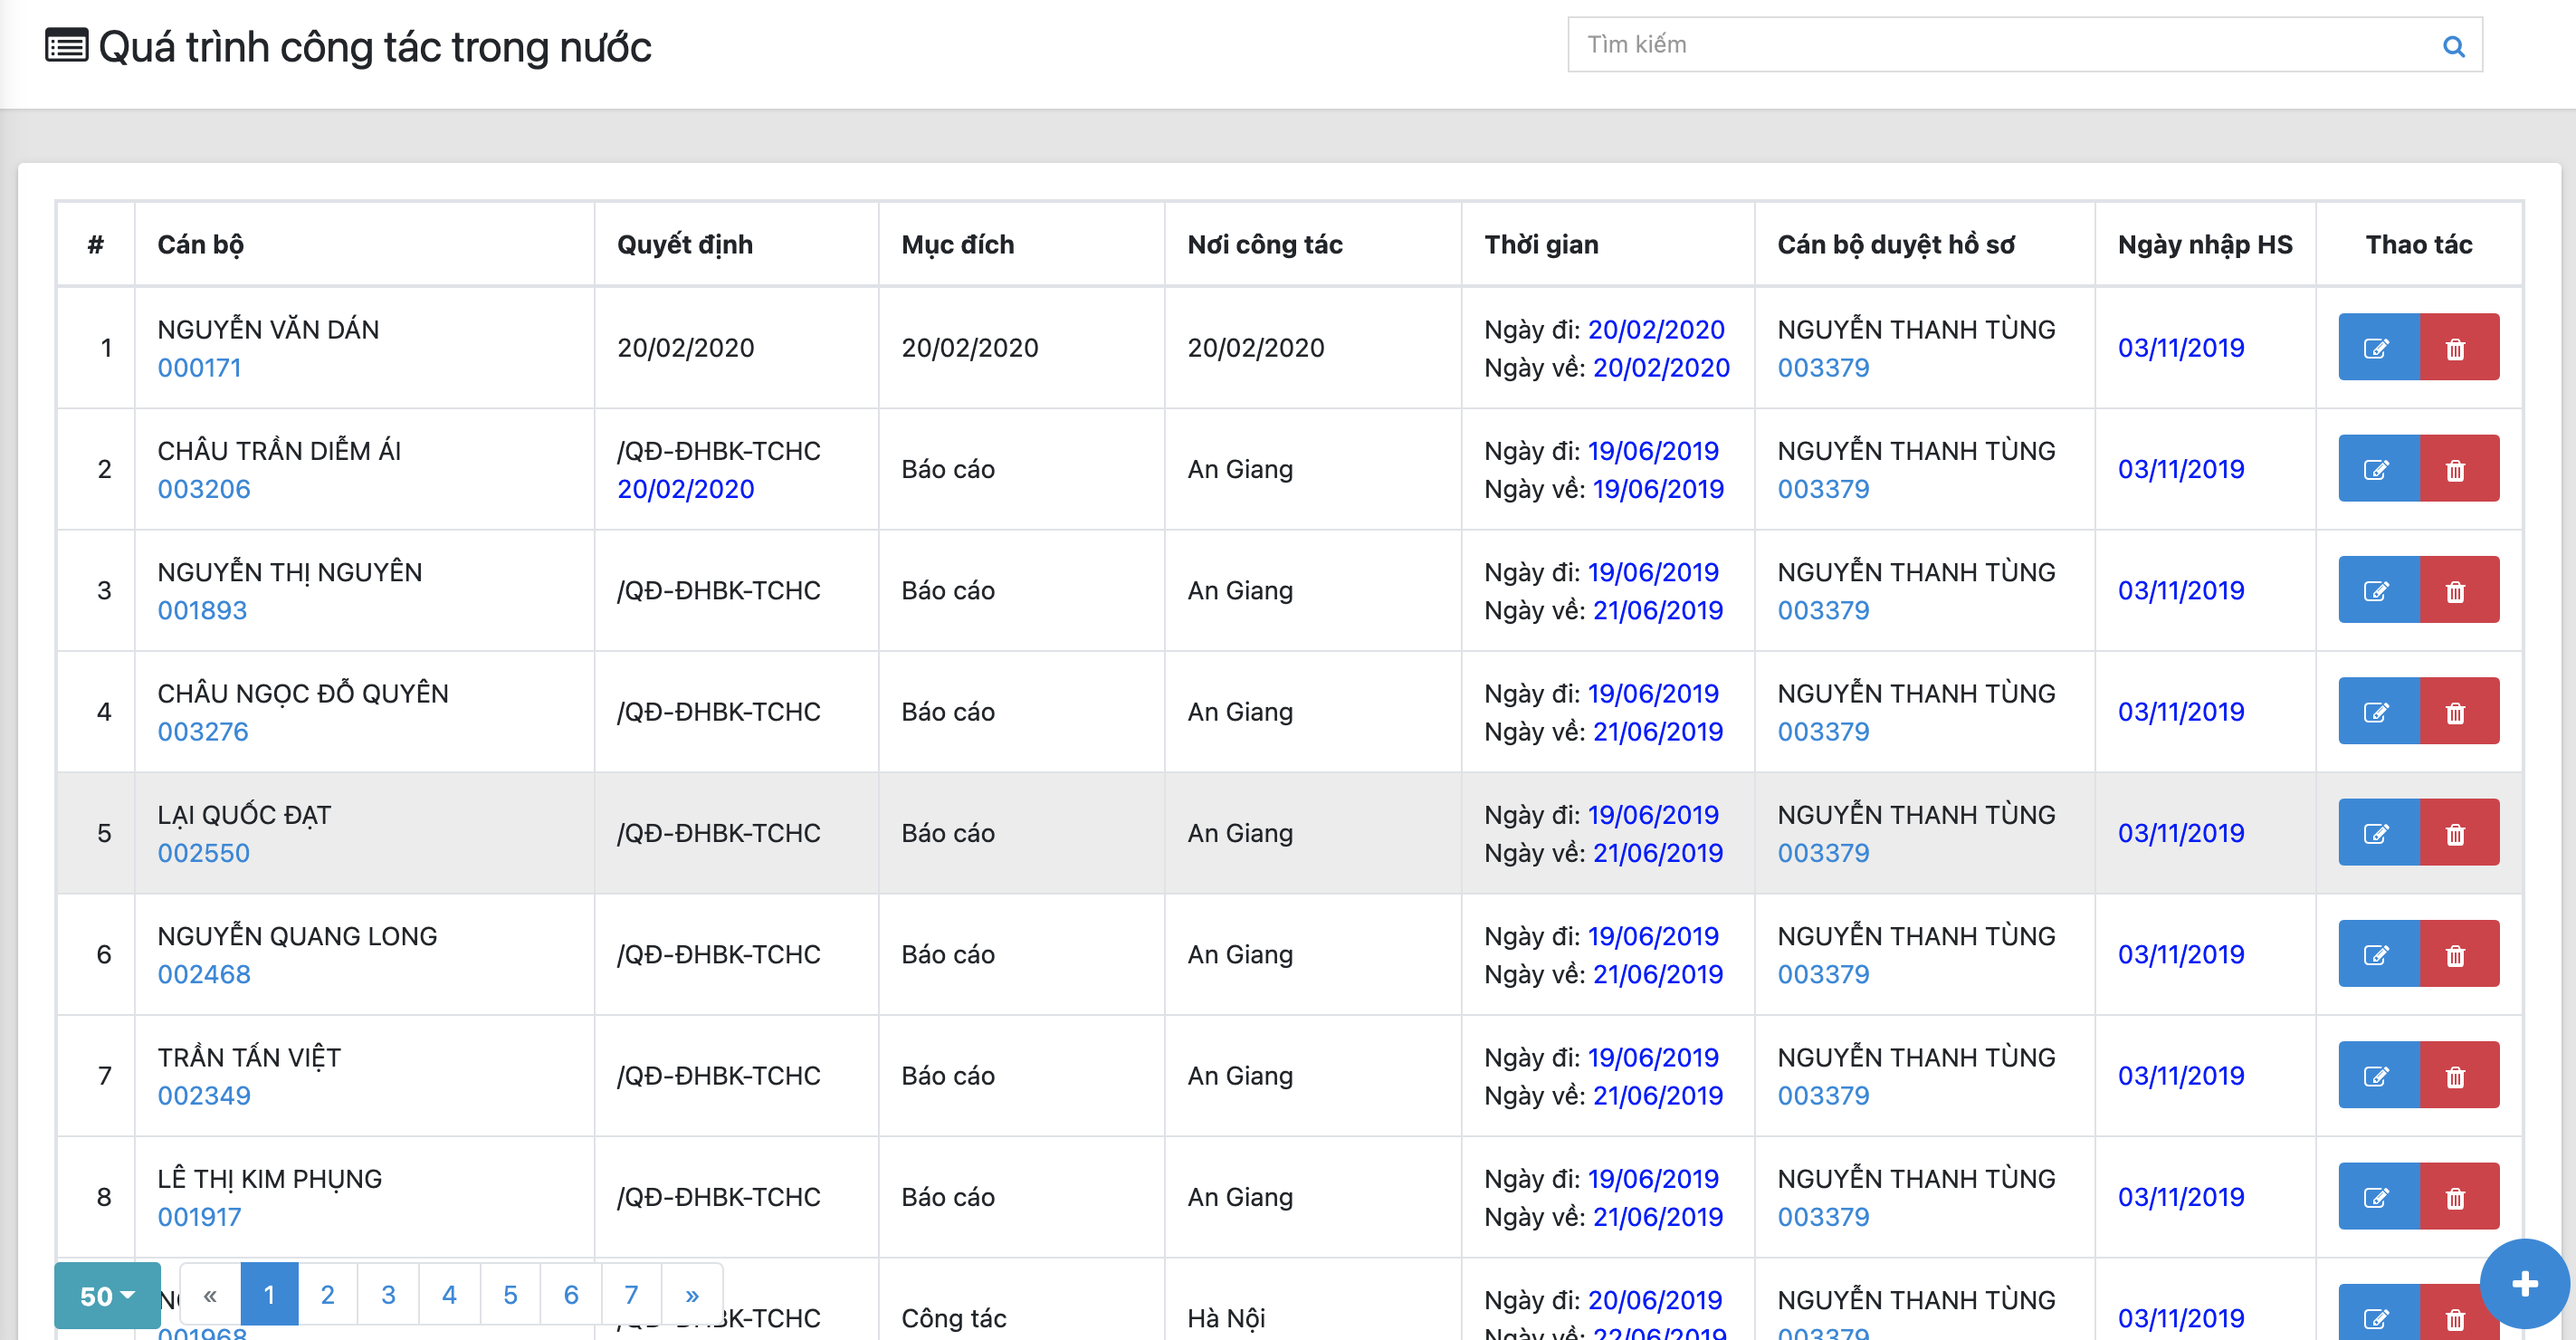
\includegraphics[width=15cm]{img/test/viewFirst.png}
  \captionof{figure}{Danh sách quá trình công tác trong nước ban đầu}
\end{center}
Tạo mới một quá trình
\begin{center}
  \captionsetup{type=figure}
  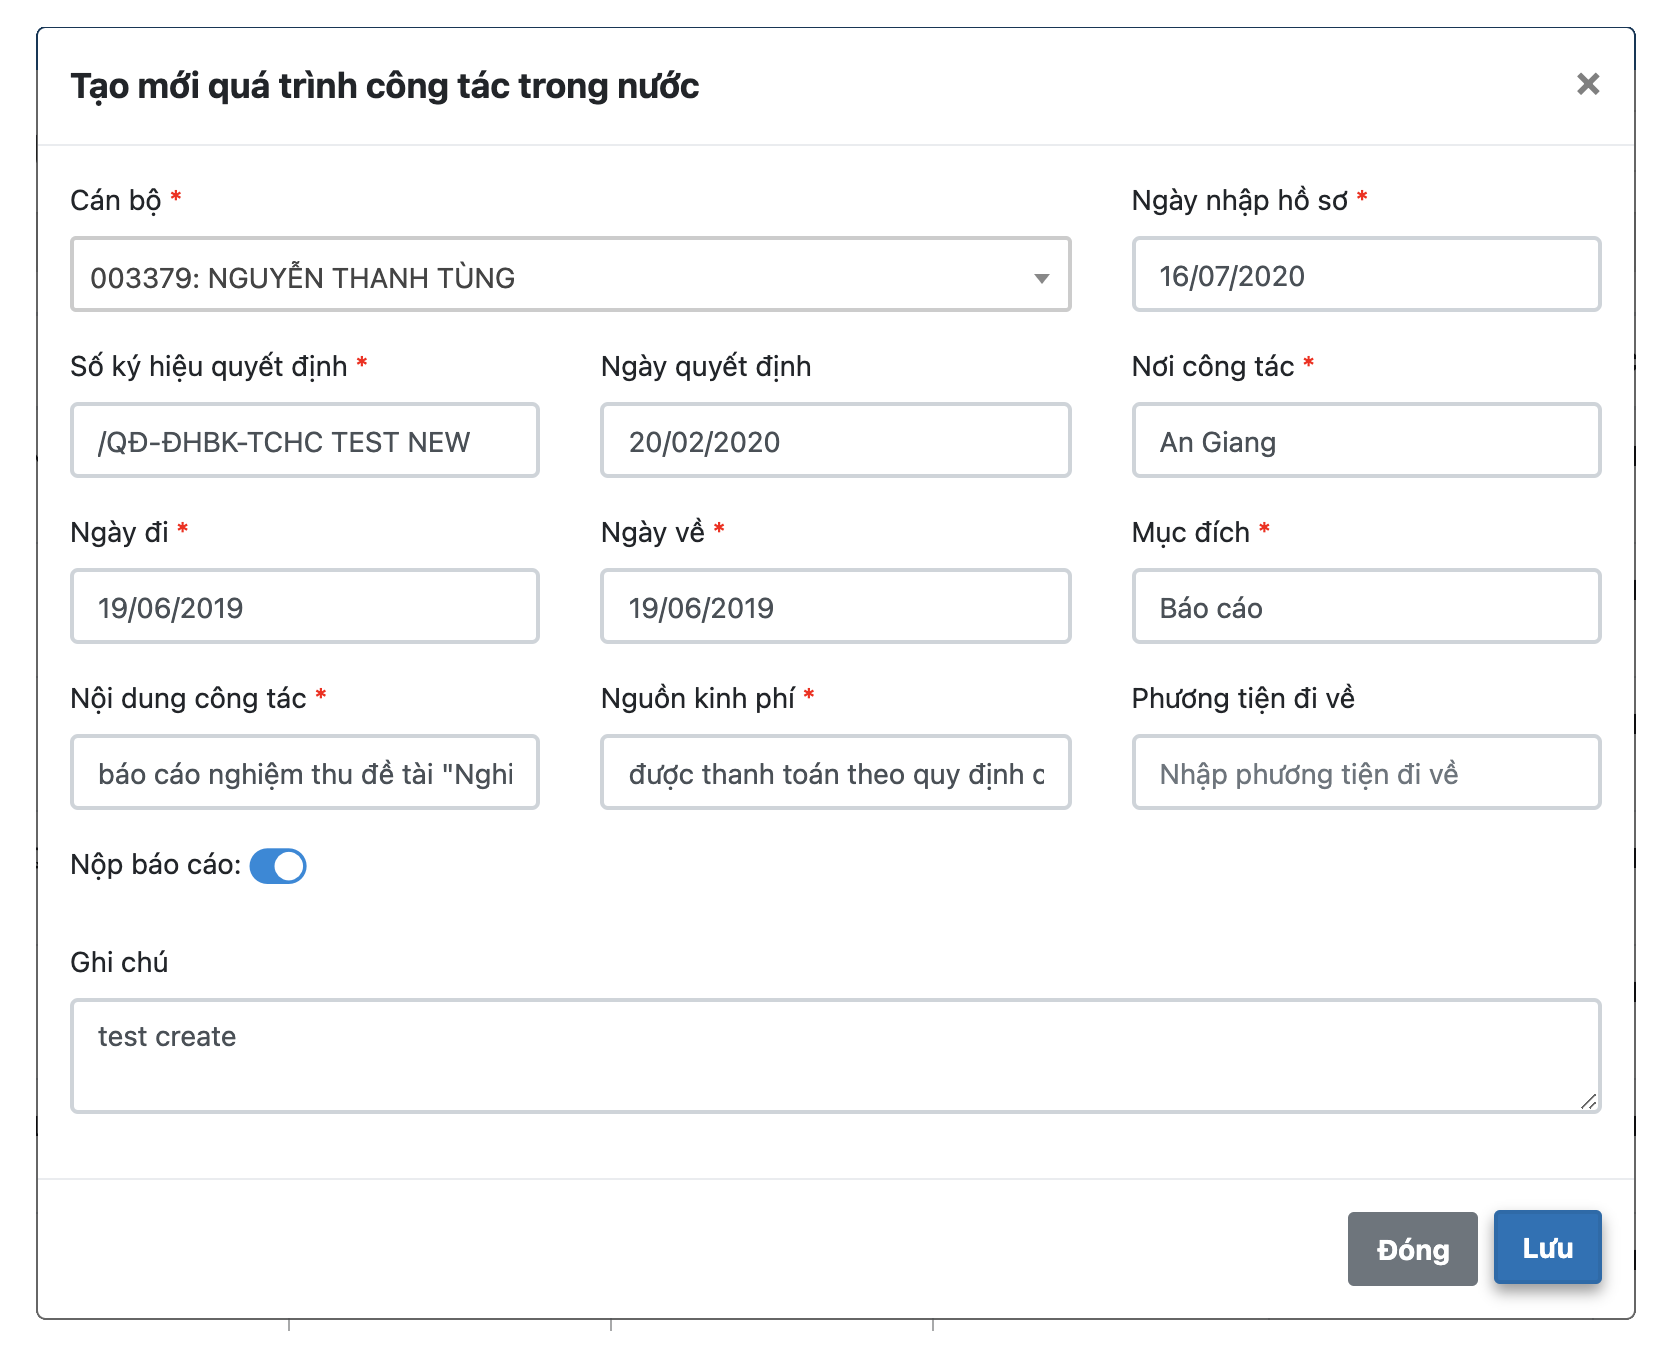
\includegraphics[width=10cm]{img/test/newForm.png}
  \captionof{figure}{Tạo mới quá tình công tác trong nước}
\end{center}
Tạo mới quá trình công tác trong nước thành công
\begin{center}
  \captionsetup{type=figure}
  
\includegraphics[width=10cm]{img/test/aleartNew.png}
  \captionof{figure}{Tạo mới quá tình công tác trong nước thành công}
\end{center}
\newpage
Quá trình mới tạo được thêm vào danh sách
\begin{center}
  \captionsetup{type=figure}
  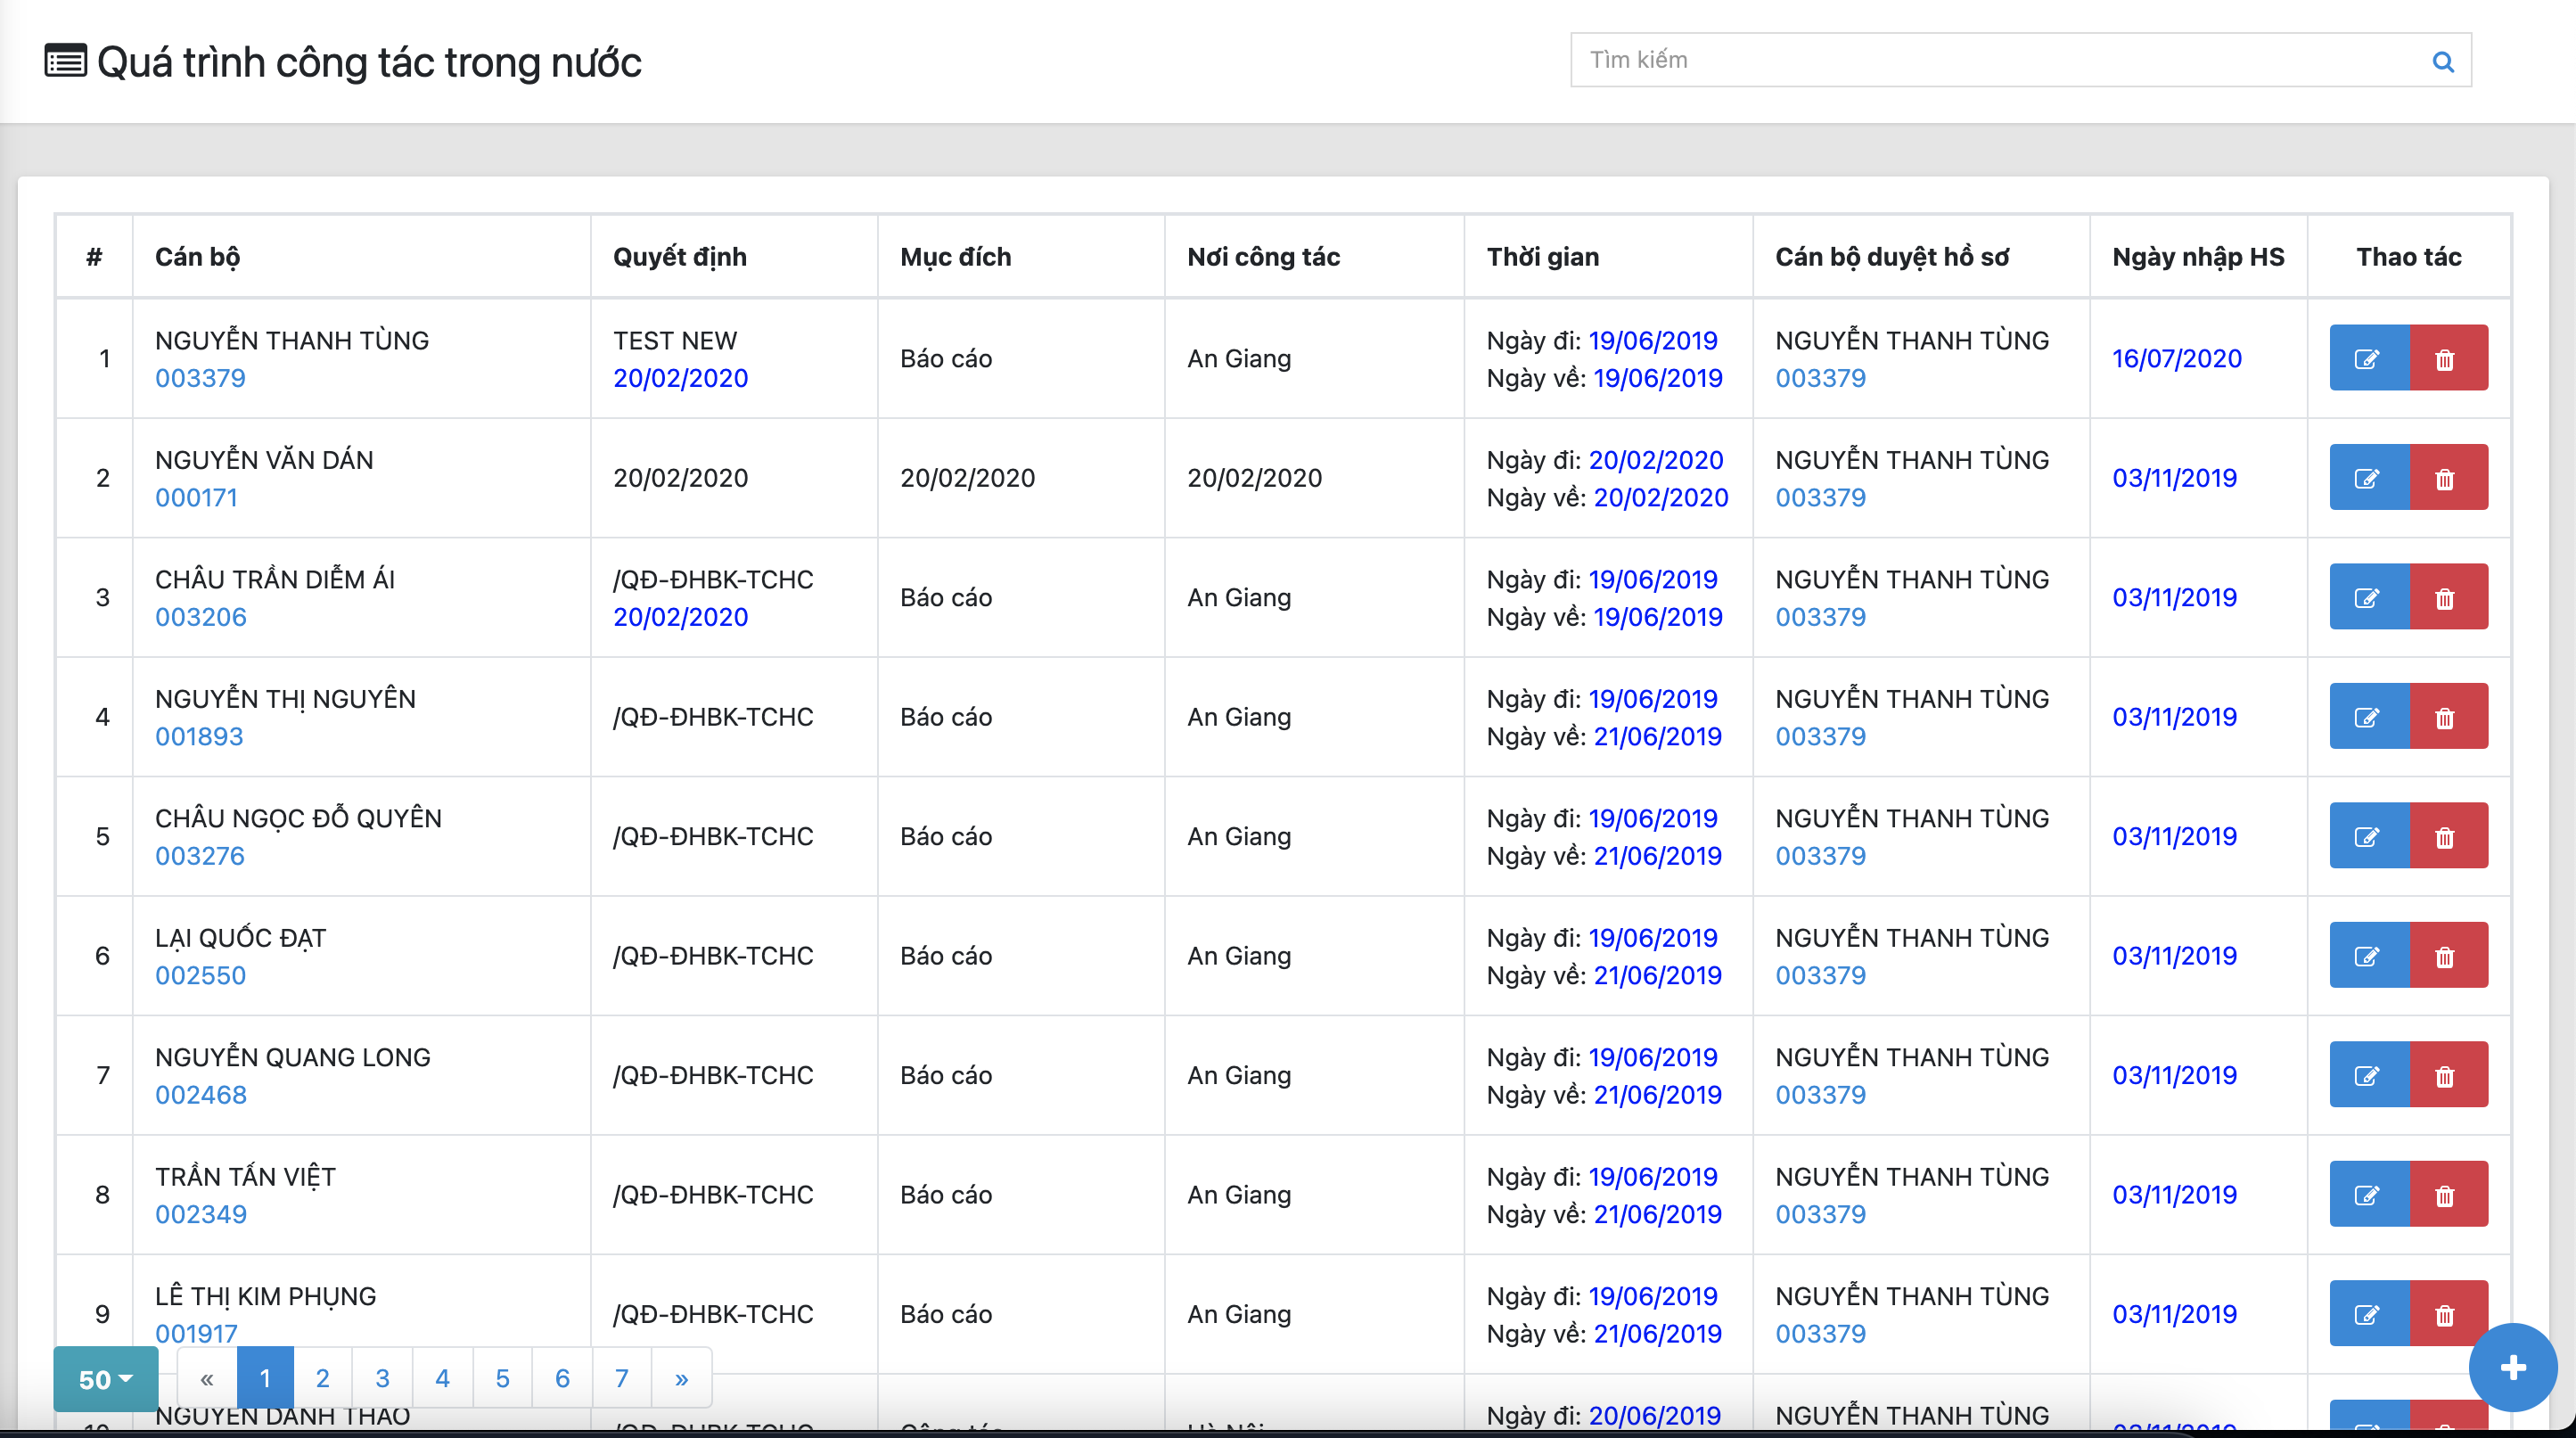
\includegraphics[width=15cm]{img/test/viewNew.png}
  \captionof{figure}{Danh sách quá trình trong nước sau khi tạo mới thành công}
\end{center}
Chỉnh sửa quá trình:
\begin{center}
  \captionsetup{type=figure}
  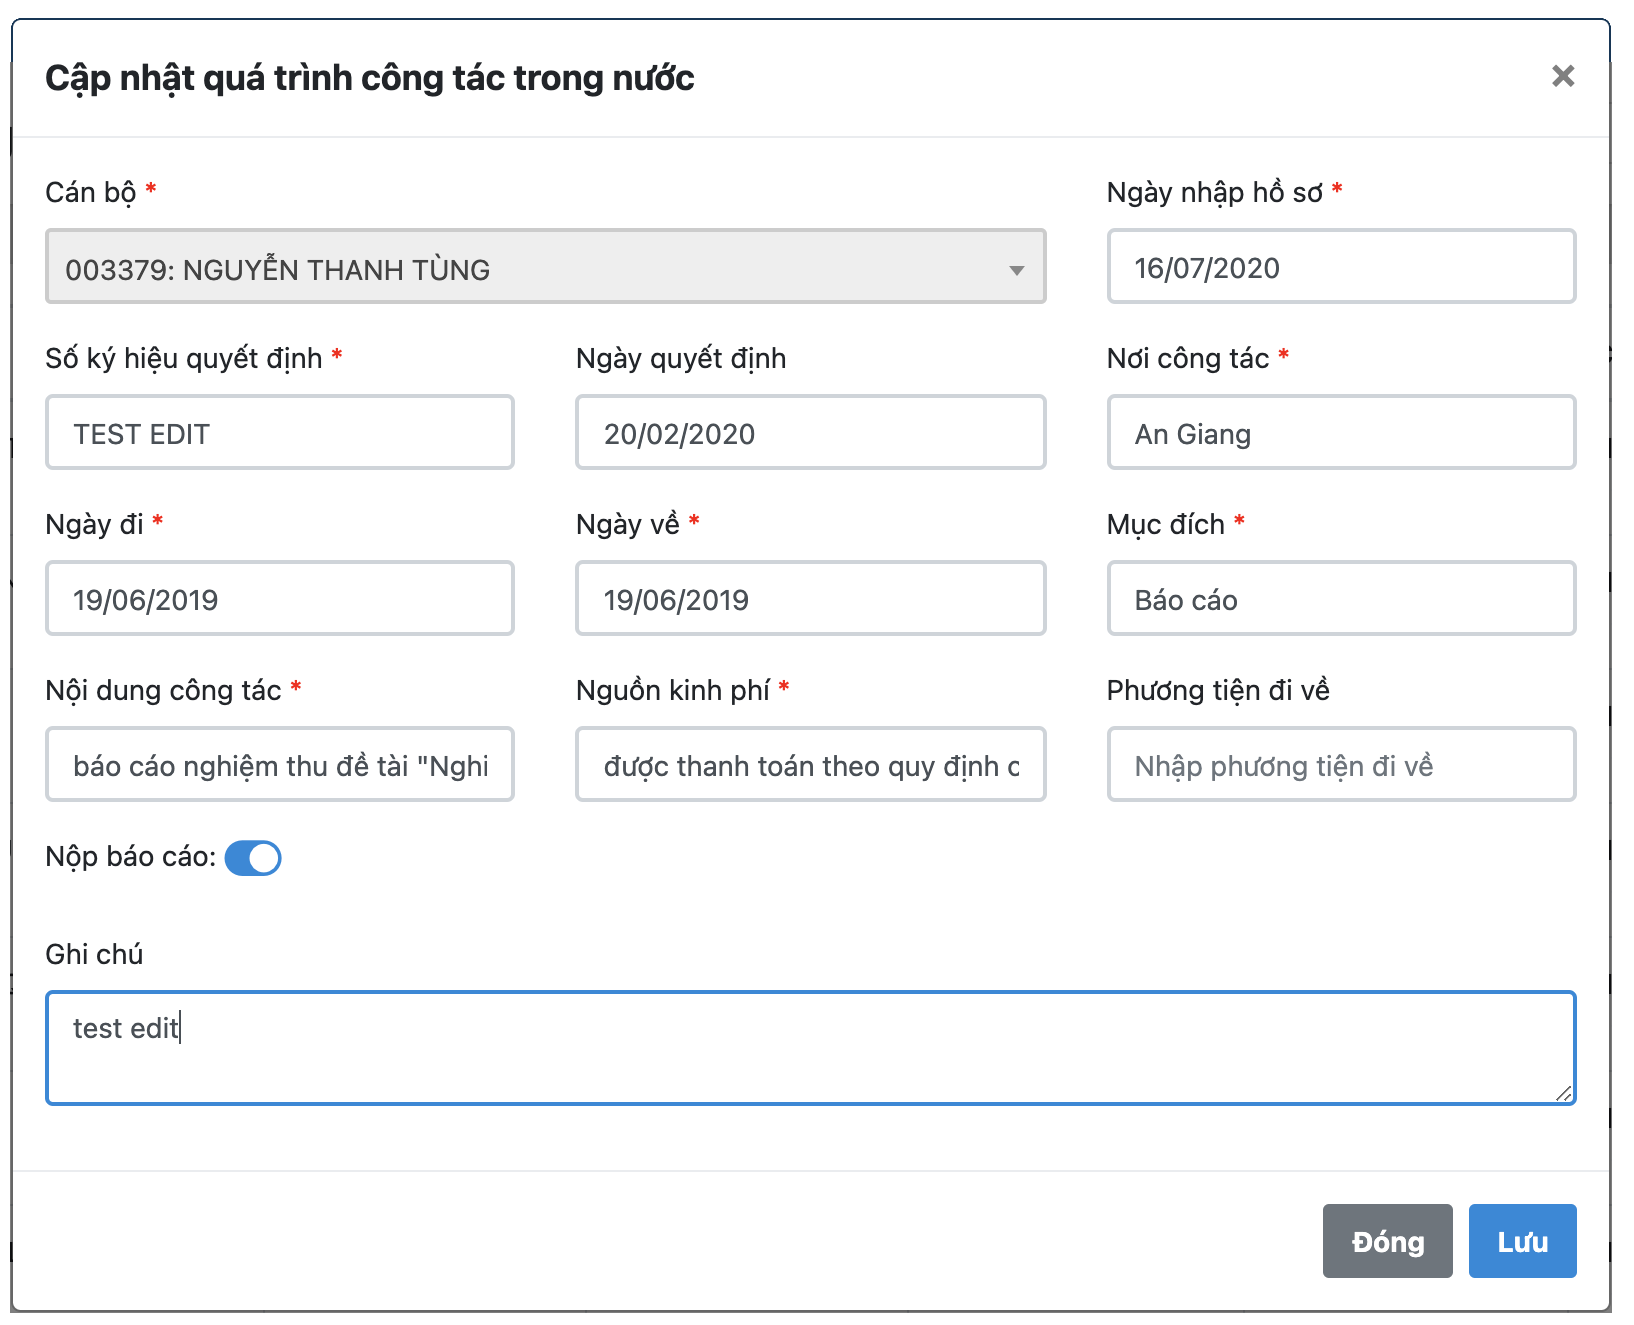
\includegraphics[width=15cm]{img/test/editForm.png}
  \captionof{figure}{Chỉnh sửa quá tình công tác trong nước}
\end{center}
Chỉnh sửa thành công:
\begin{center}
  \captionsetup{type=figure}
  
\includegraphics[width=10cm]{img/test/aleartEdit.png}
  \captionof{figure}{Chỉnh sửa quá tình công tác trong nước thành công}
\end{center}
Quá trình công tác trong nước đã được thay đổi.
\begin{center}
  \captionsetup{type=figure}
  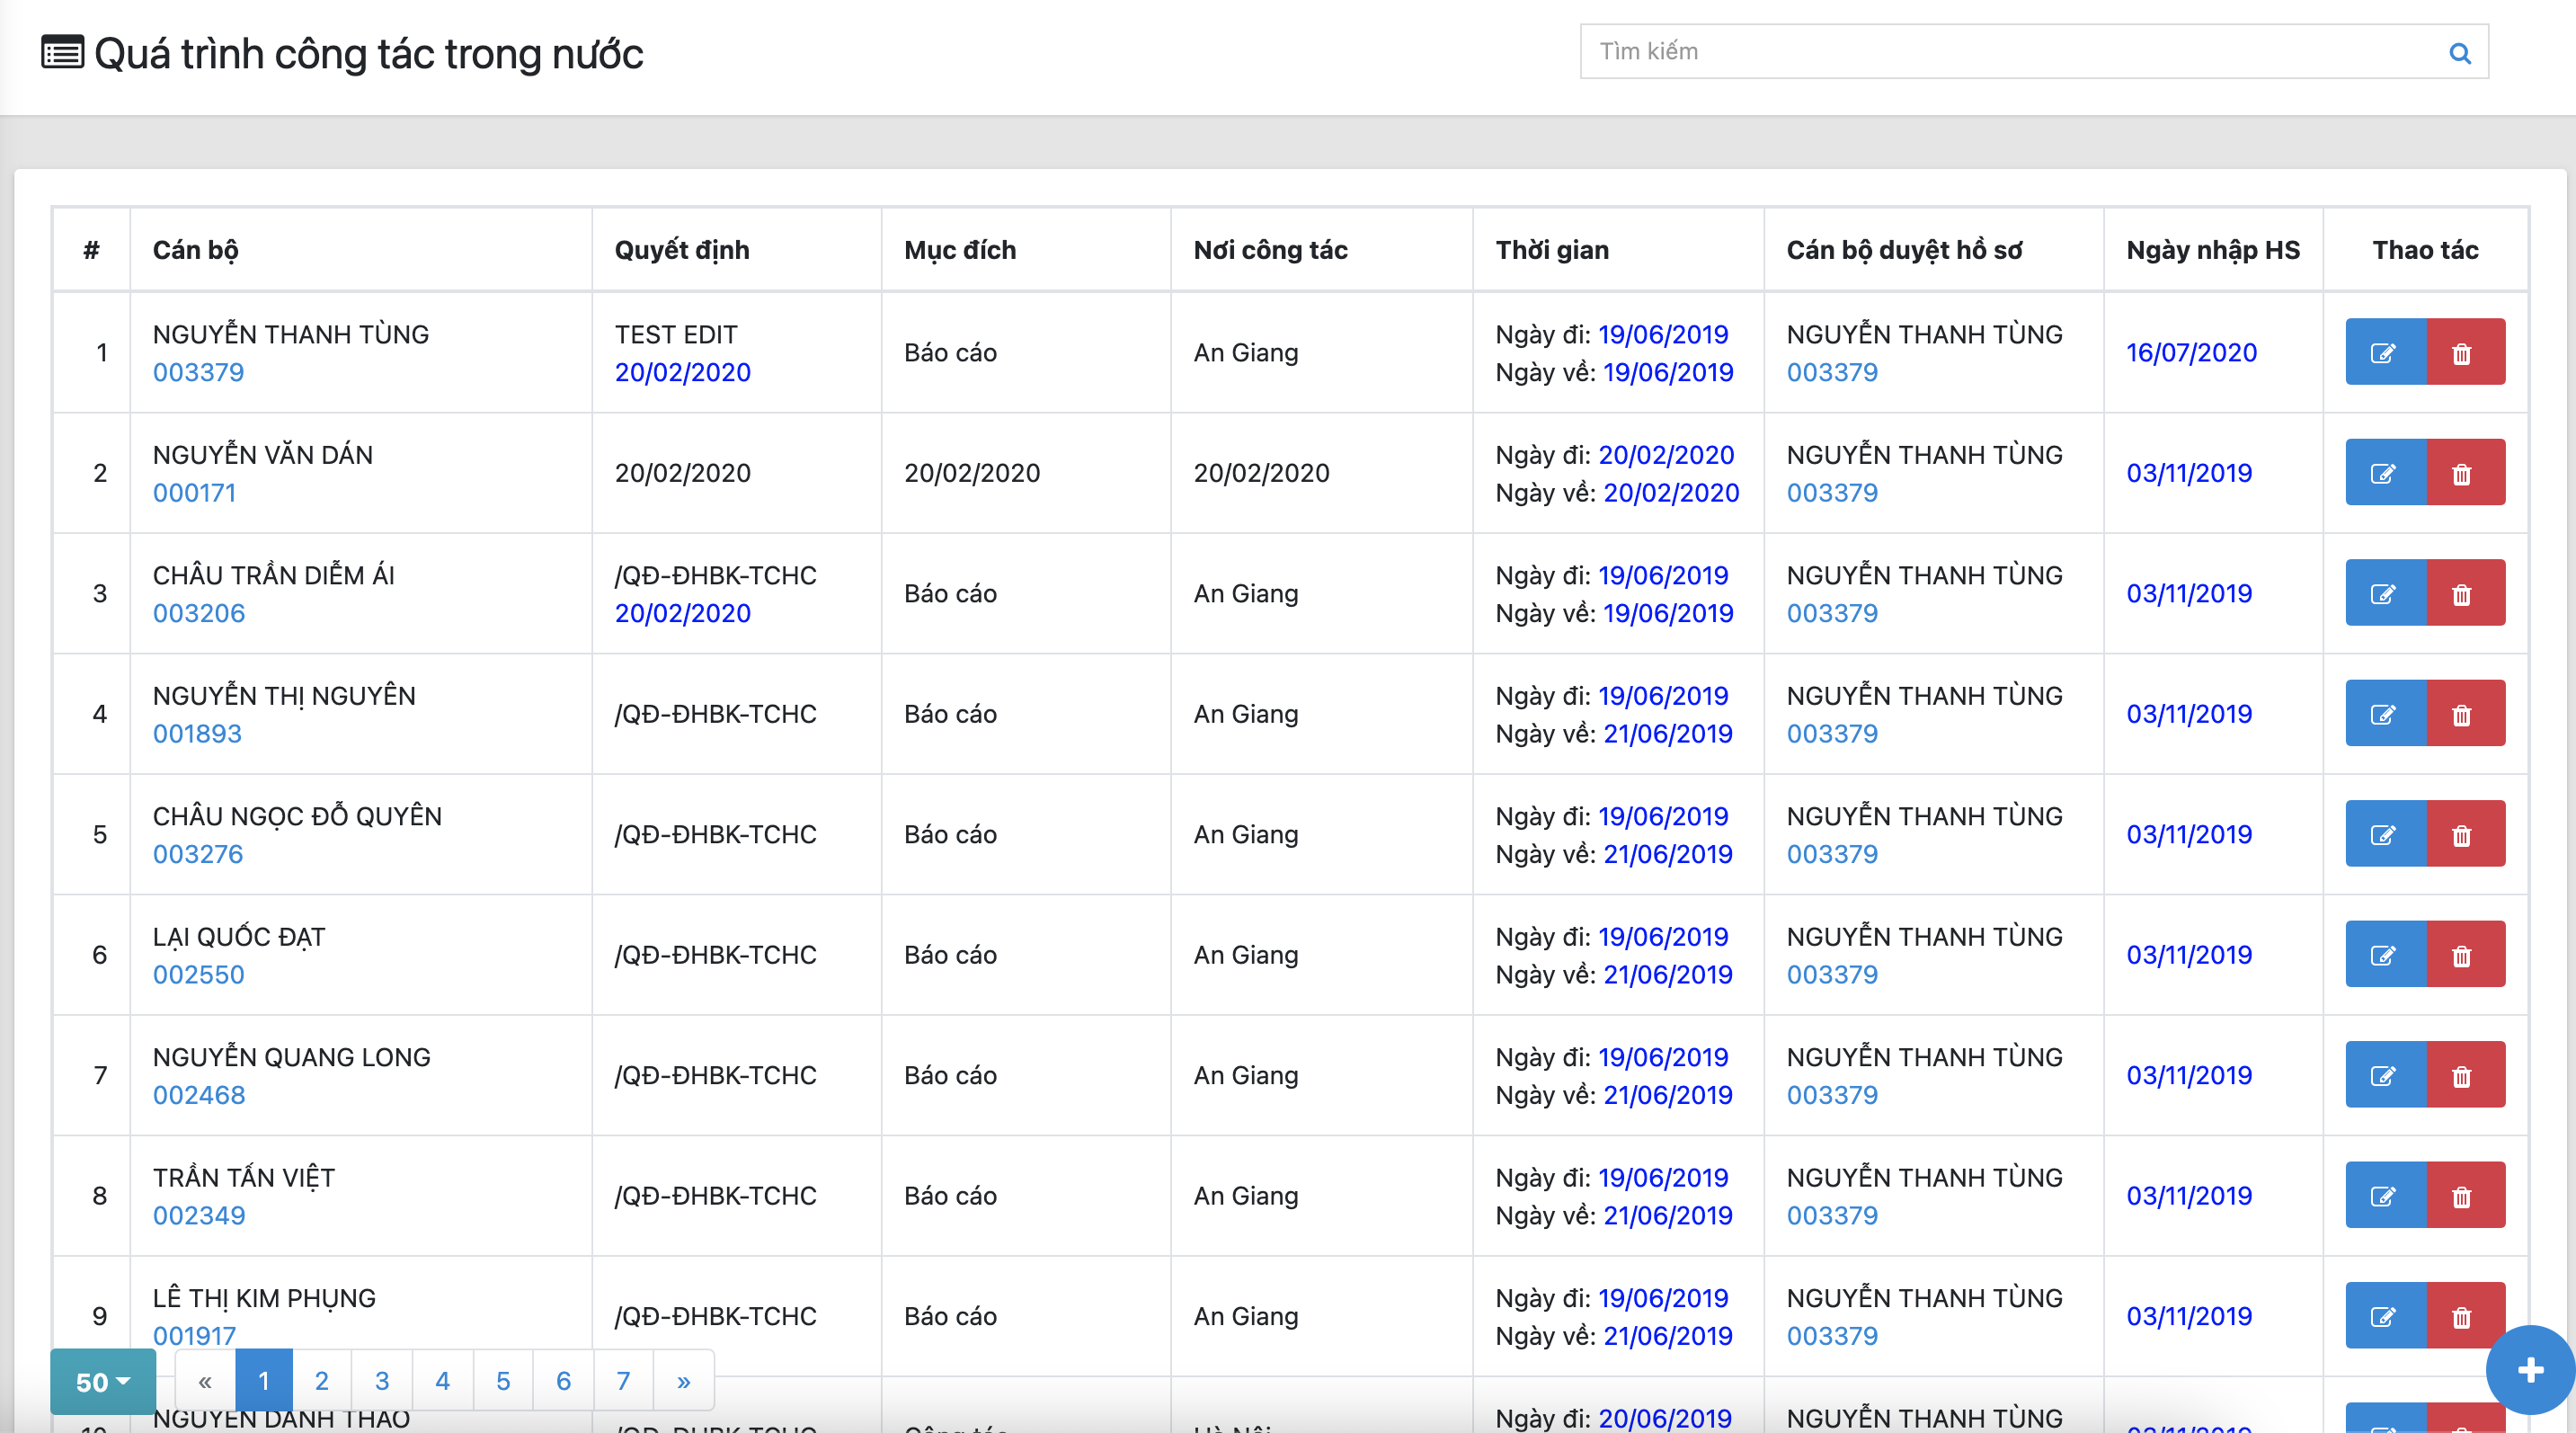
\includegraphics[width=15cm]{img/test/viewEdit.png}
  \captionof{figure}{Danh sách quá trình trong nước sau khi chỉnh sửa thành công}
\end{center}
Xoá quá trình:
\begin{center}
  \captionsetup{type=figure}
  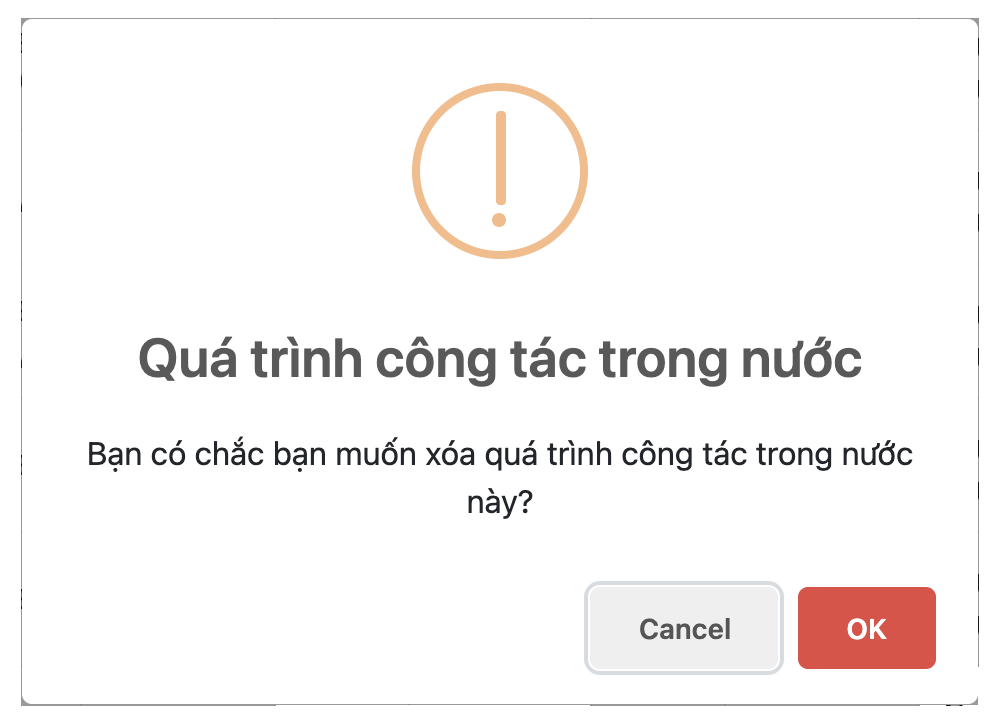
\includegraphics[width=10cm]{img/test/confirmDelete.png}
  \captionof{figure}{xác nhận xoá quá trình công tác trong nước}
\end{center}
Xoá thành công:
\begin{center}
  \captionsetup{type=figure}
  
\includegraphics[width=10cm]{img/test/aleartDelete.png}
  \captionof{figure}{Xoá quá tình công tác trong nước thành công}
\end{center}
Danh sách quá trình công tác trong nước sau khi xoá thành công
\begin{center}
  \captionsetup{type=figure}
  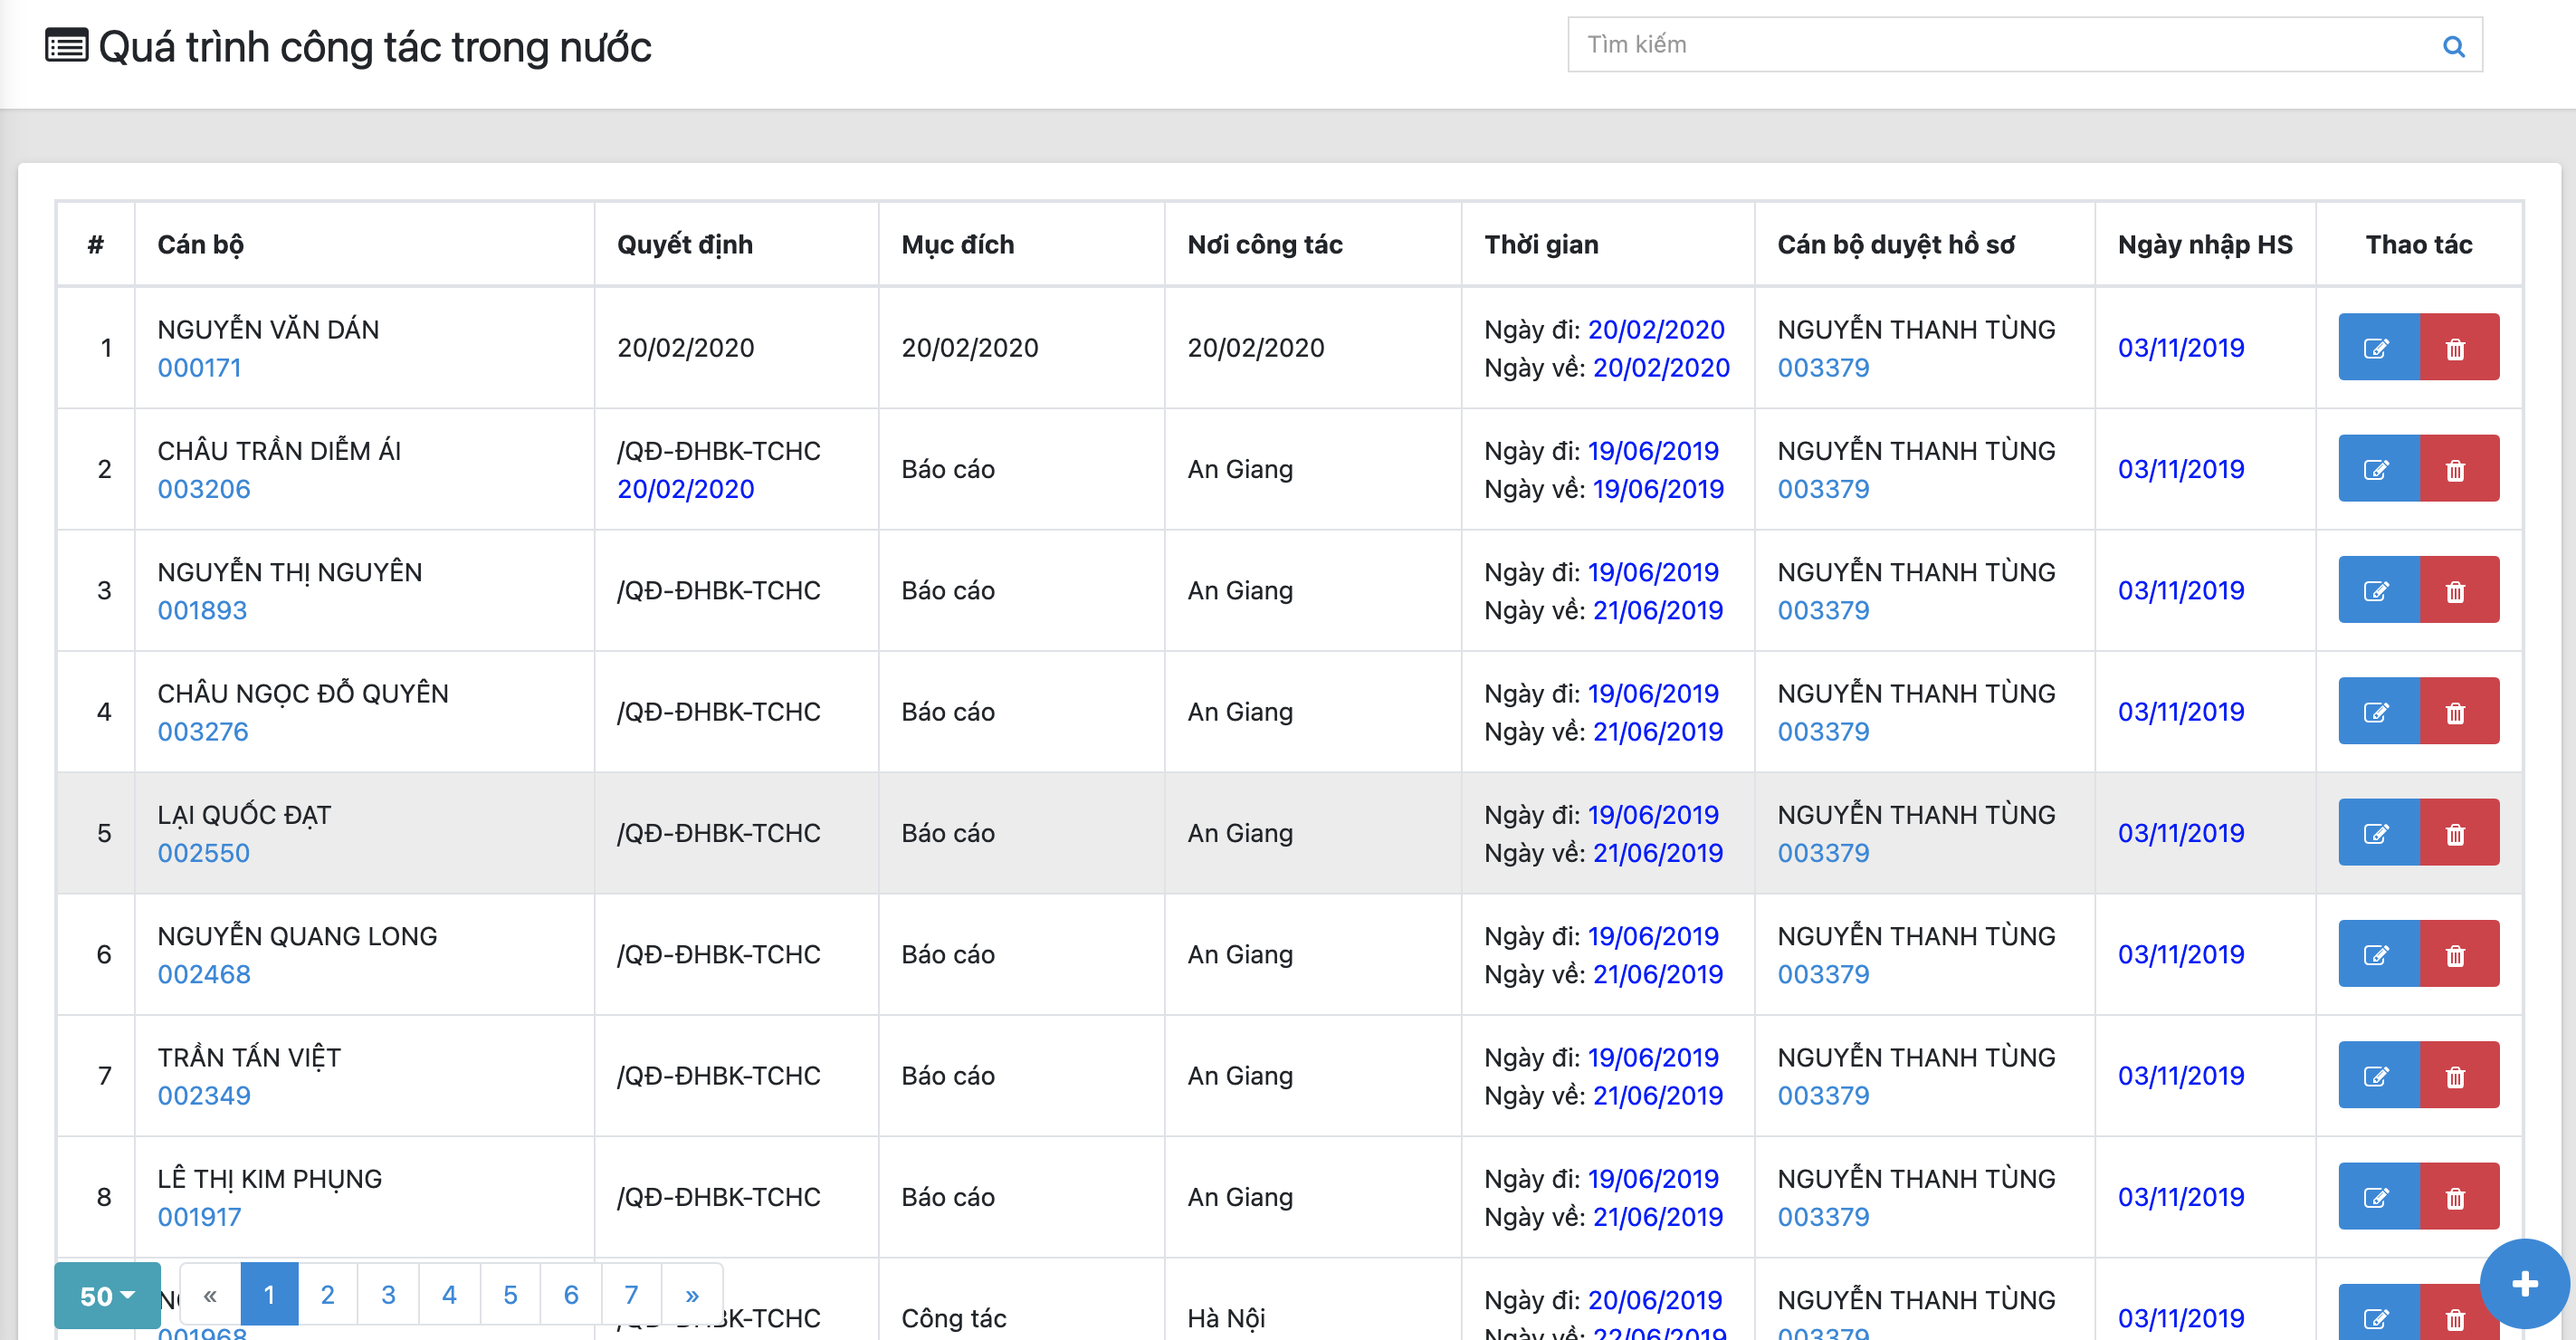
\includegraphics[width=15cm]{img/test/viewFirst.png}
  \captionof{figure}{Danh sách quá trình công tác trong nước sau khi xoá thành công}
\end{center}
\subsection{Quy trình kiểm thử tạo yêu cầu thêm, sửa, xoá quá trình với vai trò người dùng hệ thống}
Danh sách quá trình công tác trong nước của người dùng được hiển thị.
\begin{center}
  \captionsetup{type=figure}
  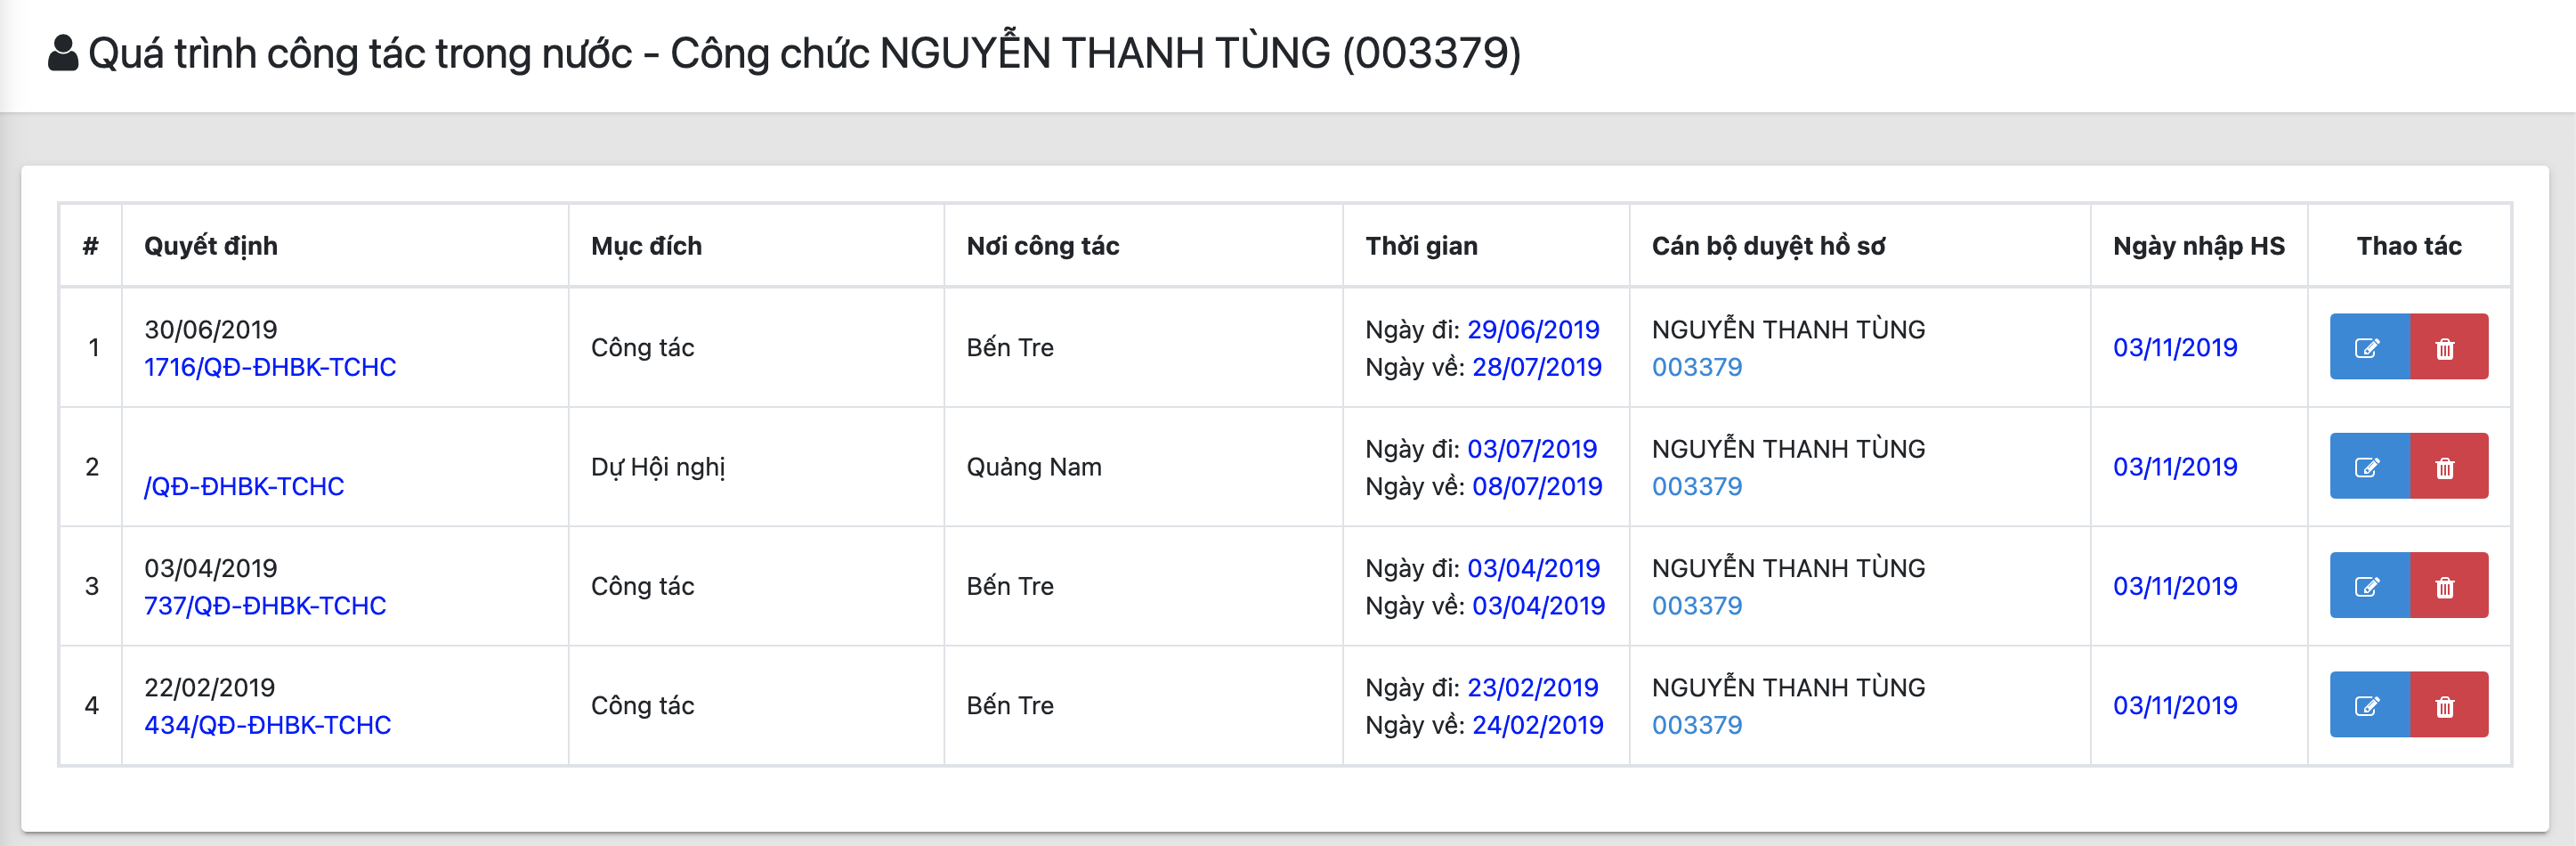
\includegraphics[width=15cm]{img/test/userView.png}
  \captionof{figure}{Danh sách quá trình công tác trong nước của người dùng}
\end{center}
Tạo yêu cầu tạo mới quá trình.
\begin{center}
  \captionsetup{type=figure}
  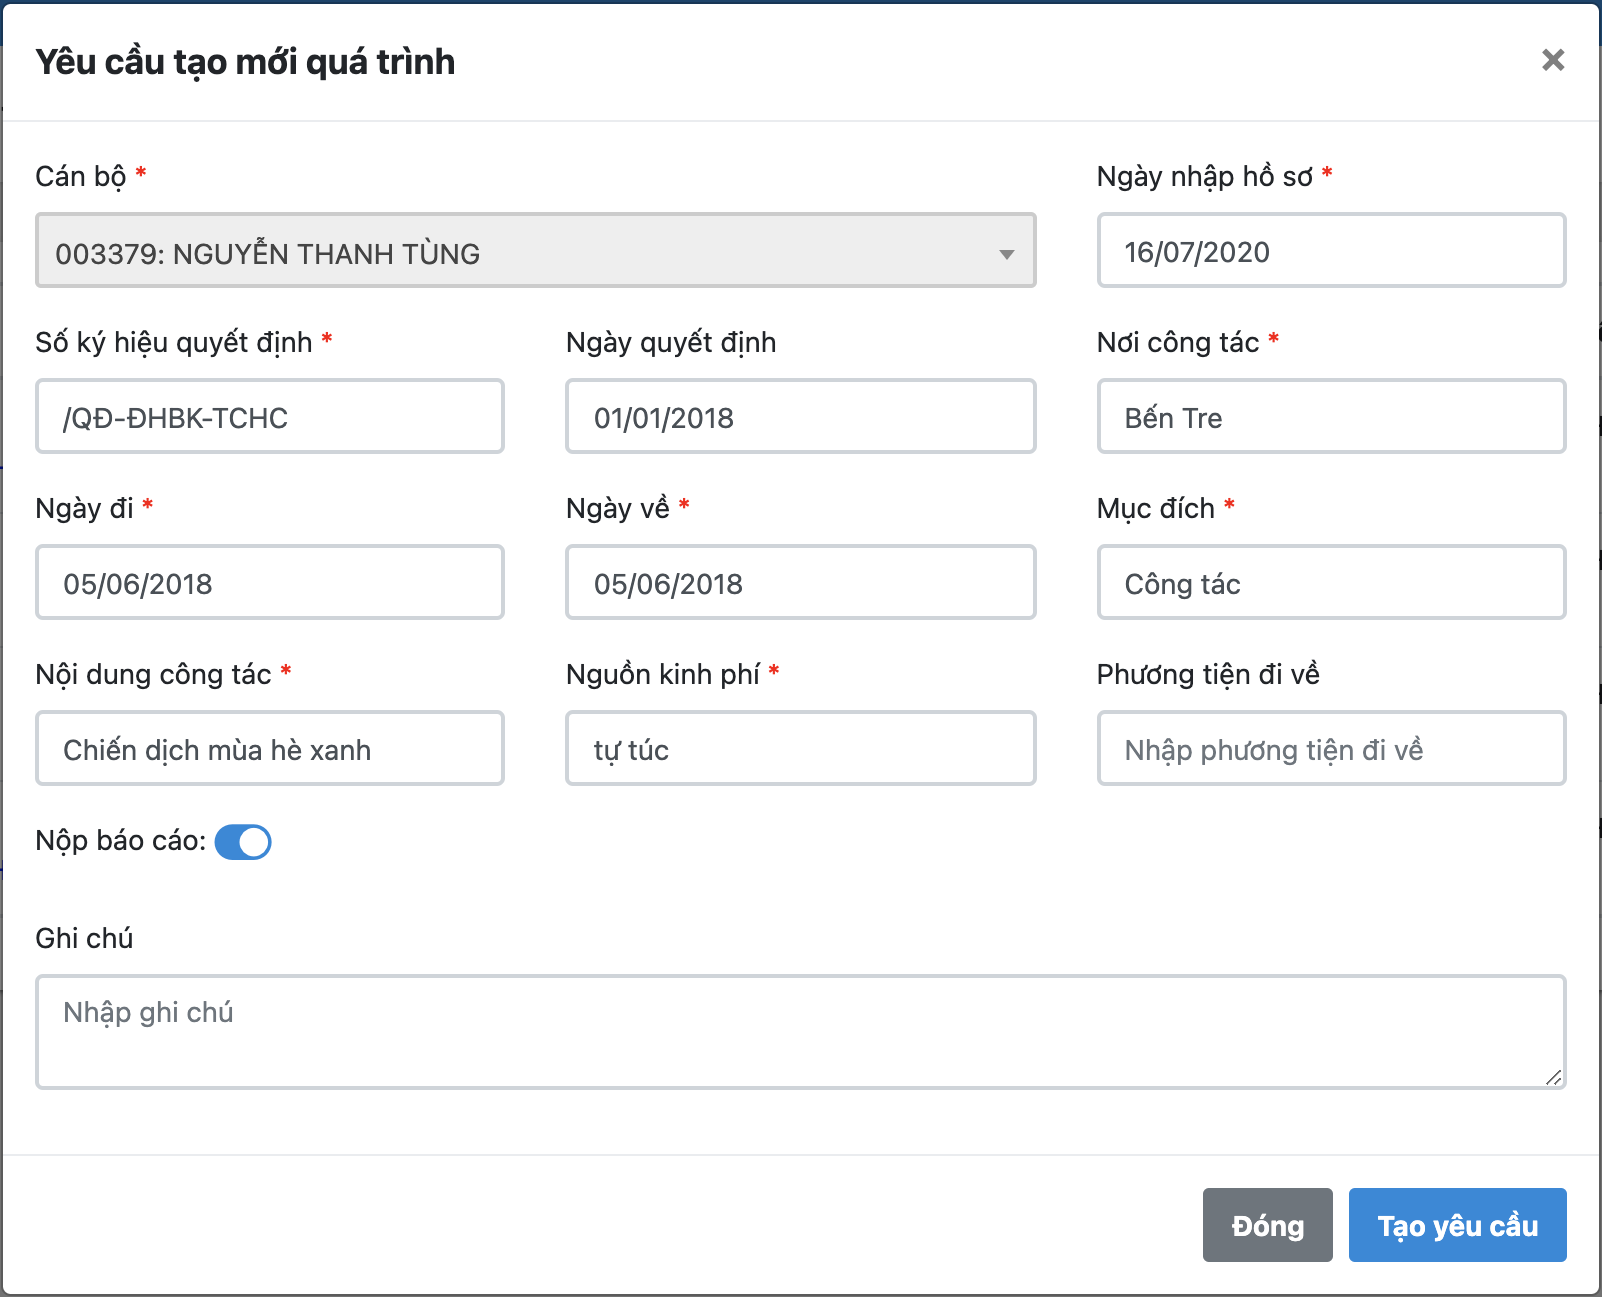
\includegraphics[width=15cm]{img/test/userForm.png}
  \captionof{figure}{Tạo yêu cầu tạo mới quá trình công tác trong nước}
\end{center}
Yêu cầu được thêm vào danh sách yêu cầu
\begin{center}
  \captionsetup{type=figure}
  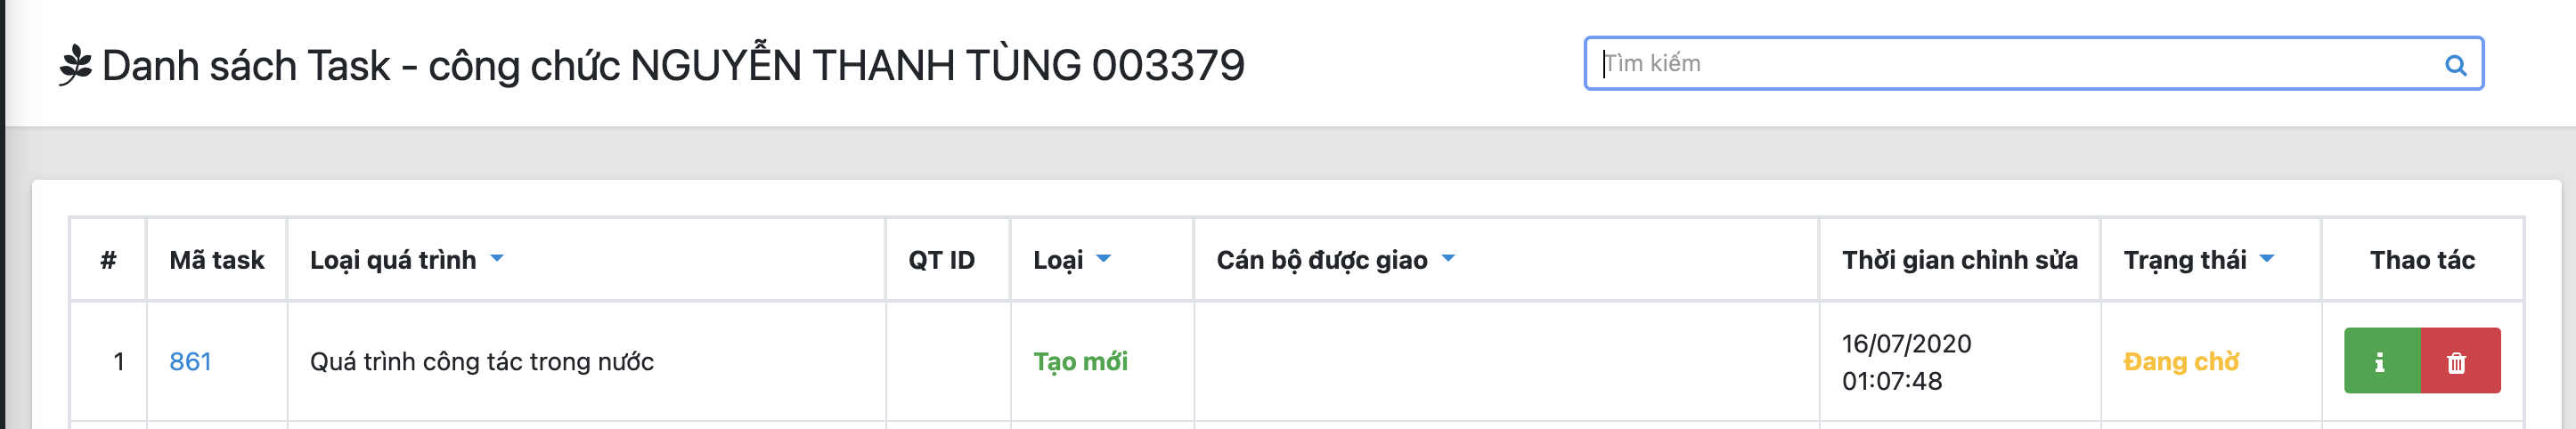
\includegraphics[width=15cm]{img/test/userTask.png}
  \captionof{figure}{Danh sách các yêu cầu của cá nhân người dùng}
\end{center}
Xem chi tiết và chỉnh sửa lại yêu cầu
\begin{center}
  \captionsetup{type=figure}
  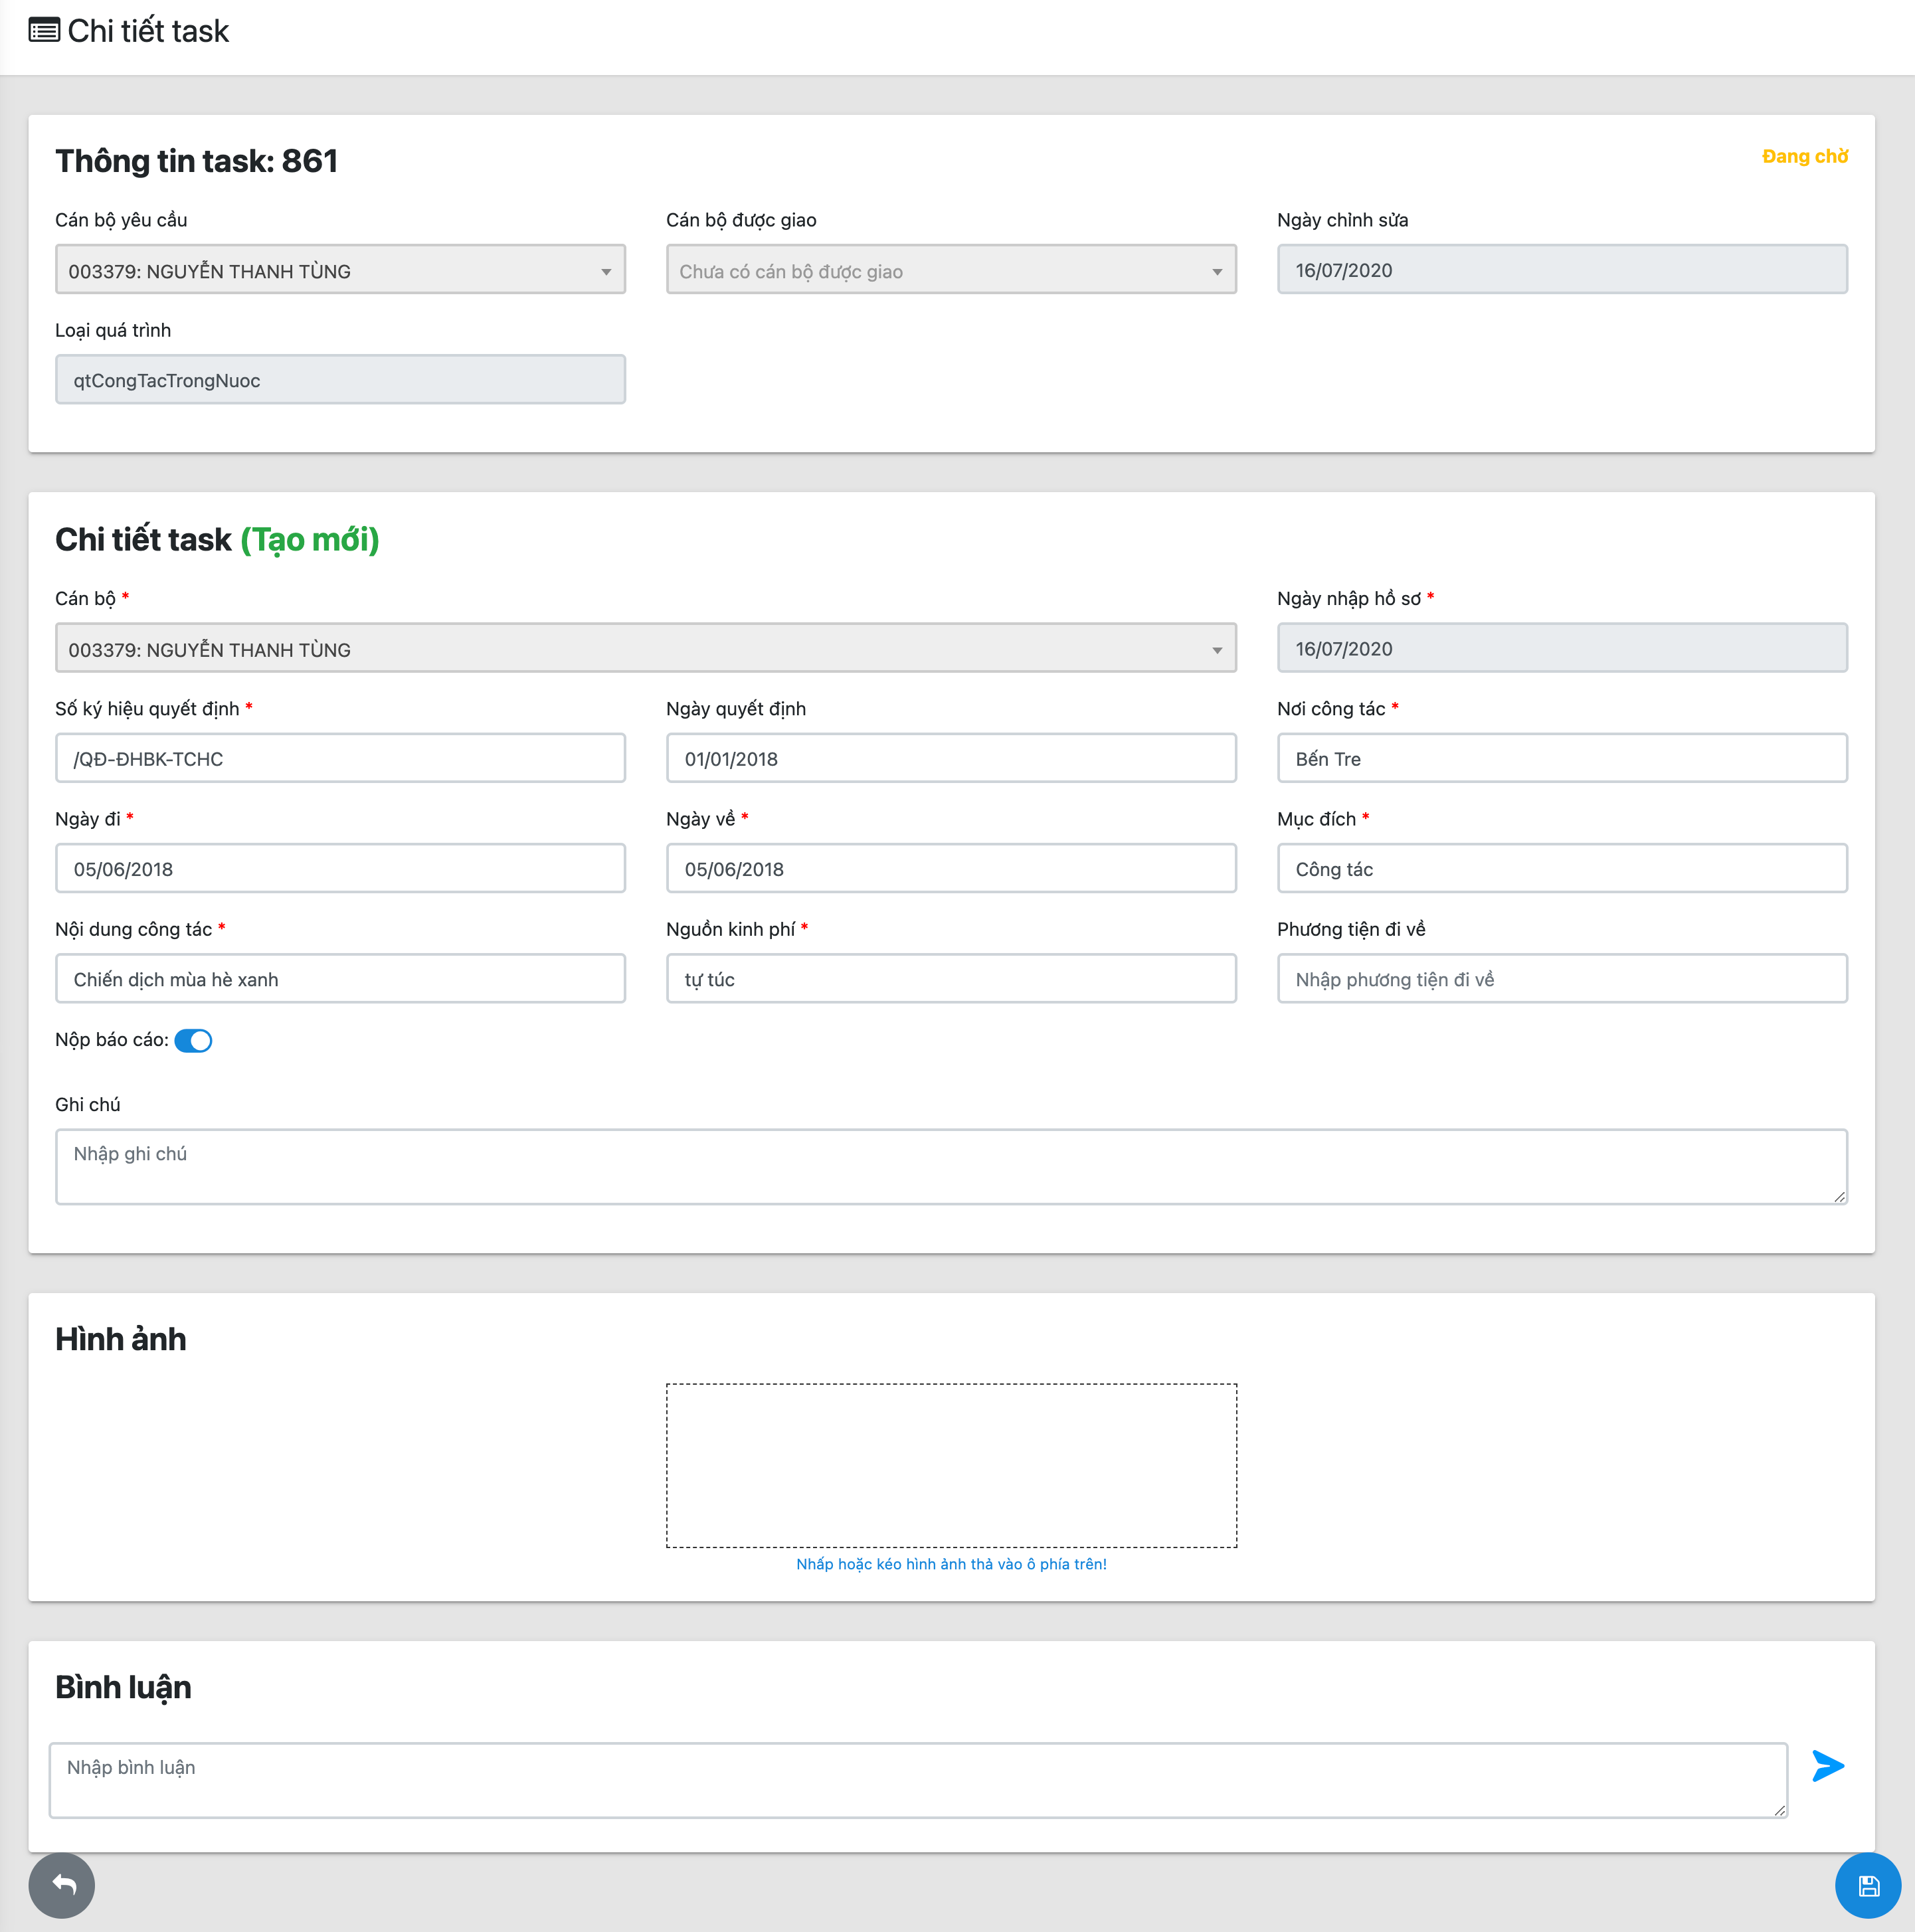
\includegraphics[width=15cm]{img/test/taskDetailUser.png}
  \captionof{figure}{Chi tiết yêu cầu của người dùng}
\end{center}
\subsection{Quy trình kiểm thử duyệt yêu cầu với vai trò cán bộ phòng Tổ chức-Hành chính}
Xem danh sách các yêu cầu
\begin{center}
  \captionsetup{type=figure}
  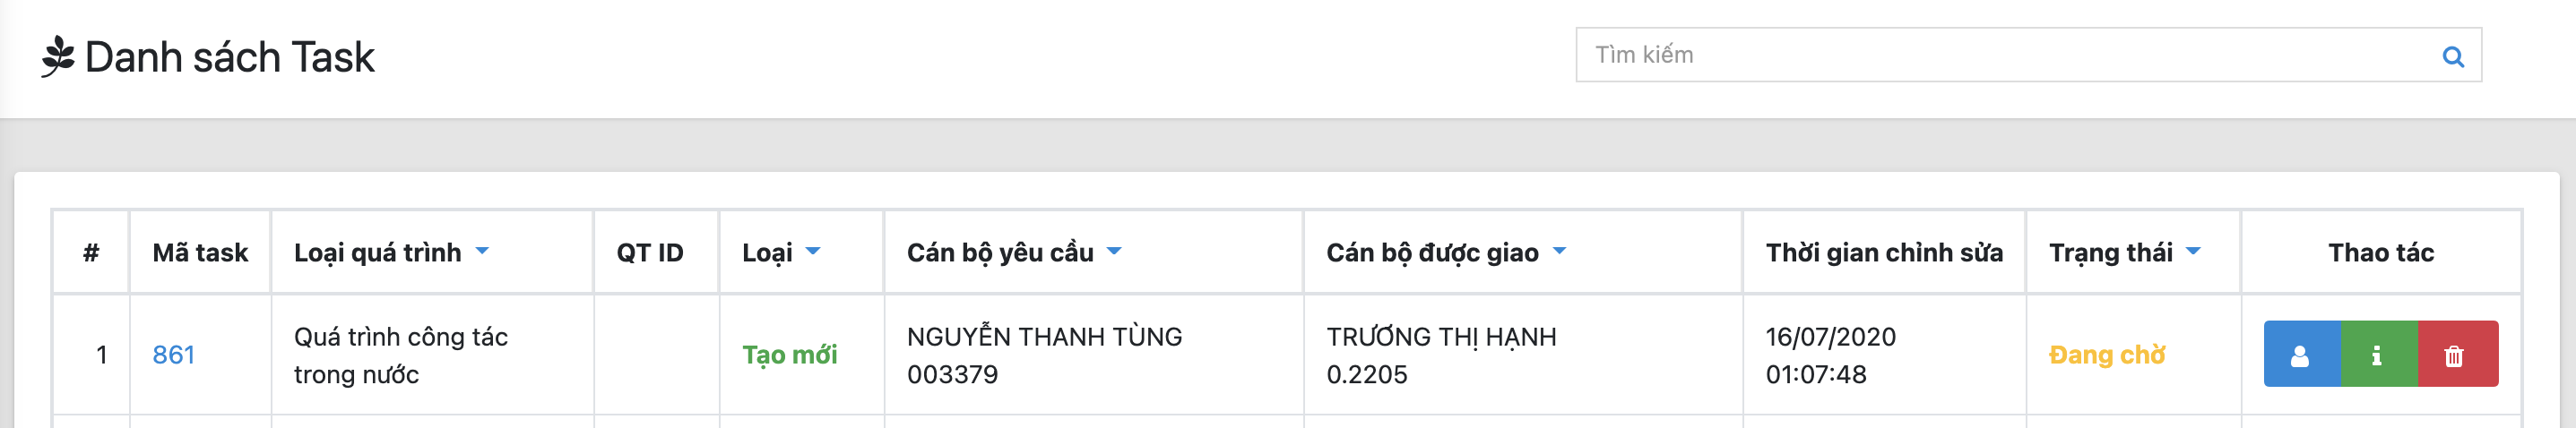
\includegraphics[width=15cm]{img/test/adminTask.png}
  \captionof{figure}{Danh sách các yêu cầu của tất cả người dùng}
\end{center}

\newpage Trưởng phòng giao yêu cầu cho cán bộ để xem xét
\begin{center}
  \captionsetup{type=figure}
  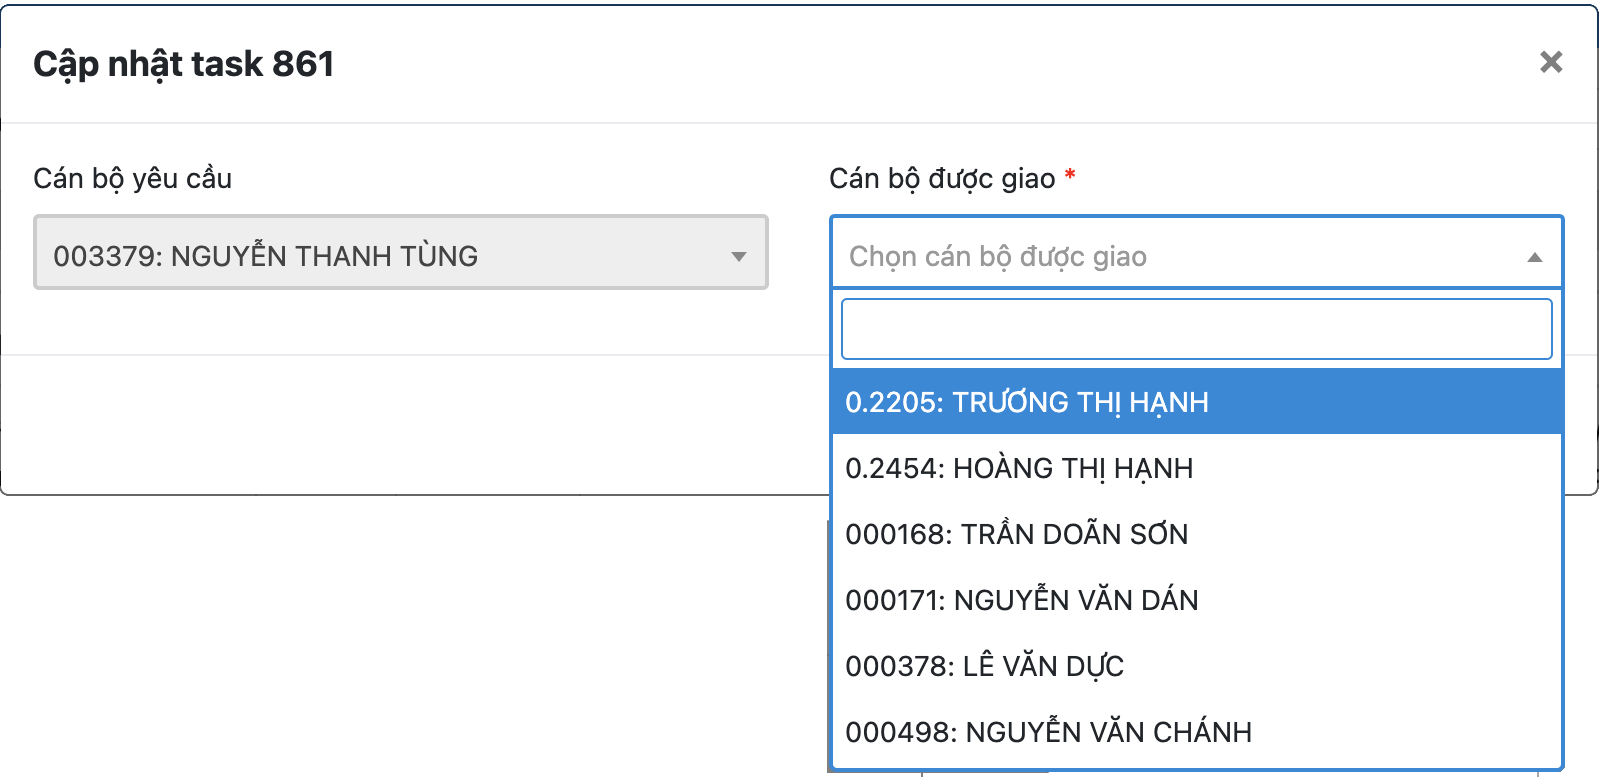
\includegraphics[width=15cm]{img/test/assignAdmin.png}
  \captionof{figure}{Giao yêu cầu cho cán bộ phòng Tổ chức - Hành chính xử lý}
\end{center}
Xem thông tin chi tiết yêu cầu
\begin{center}
  \captionsetup{type=figure}
  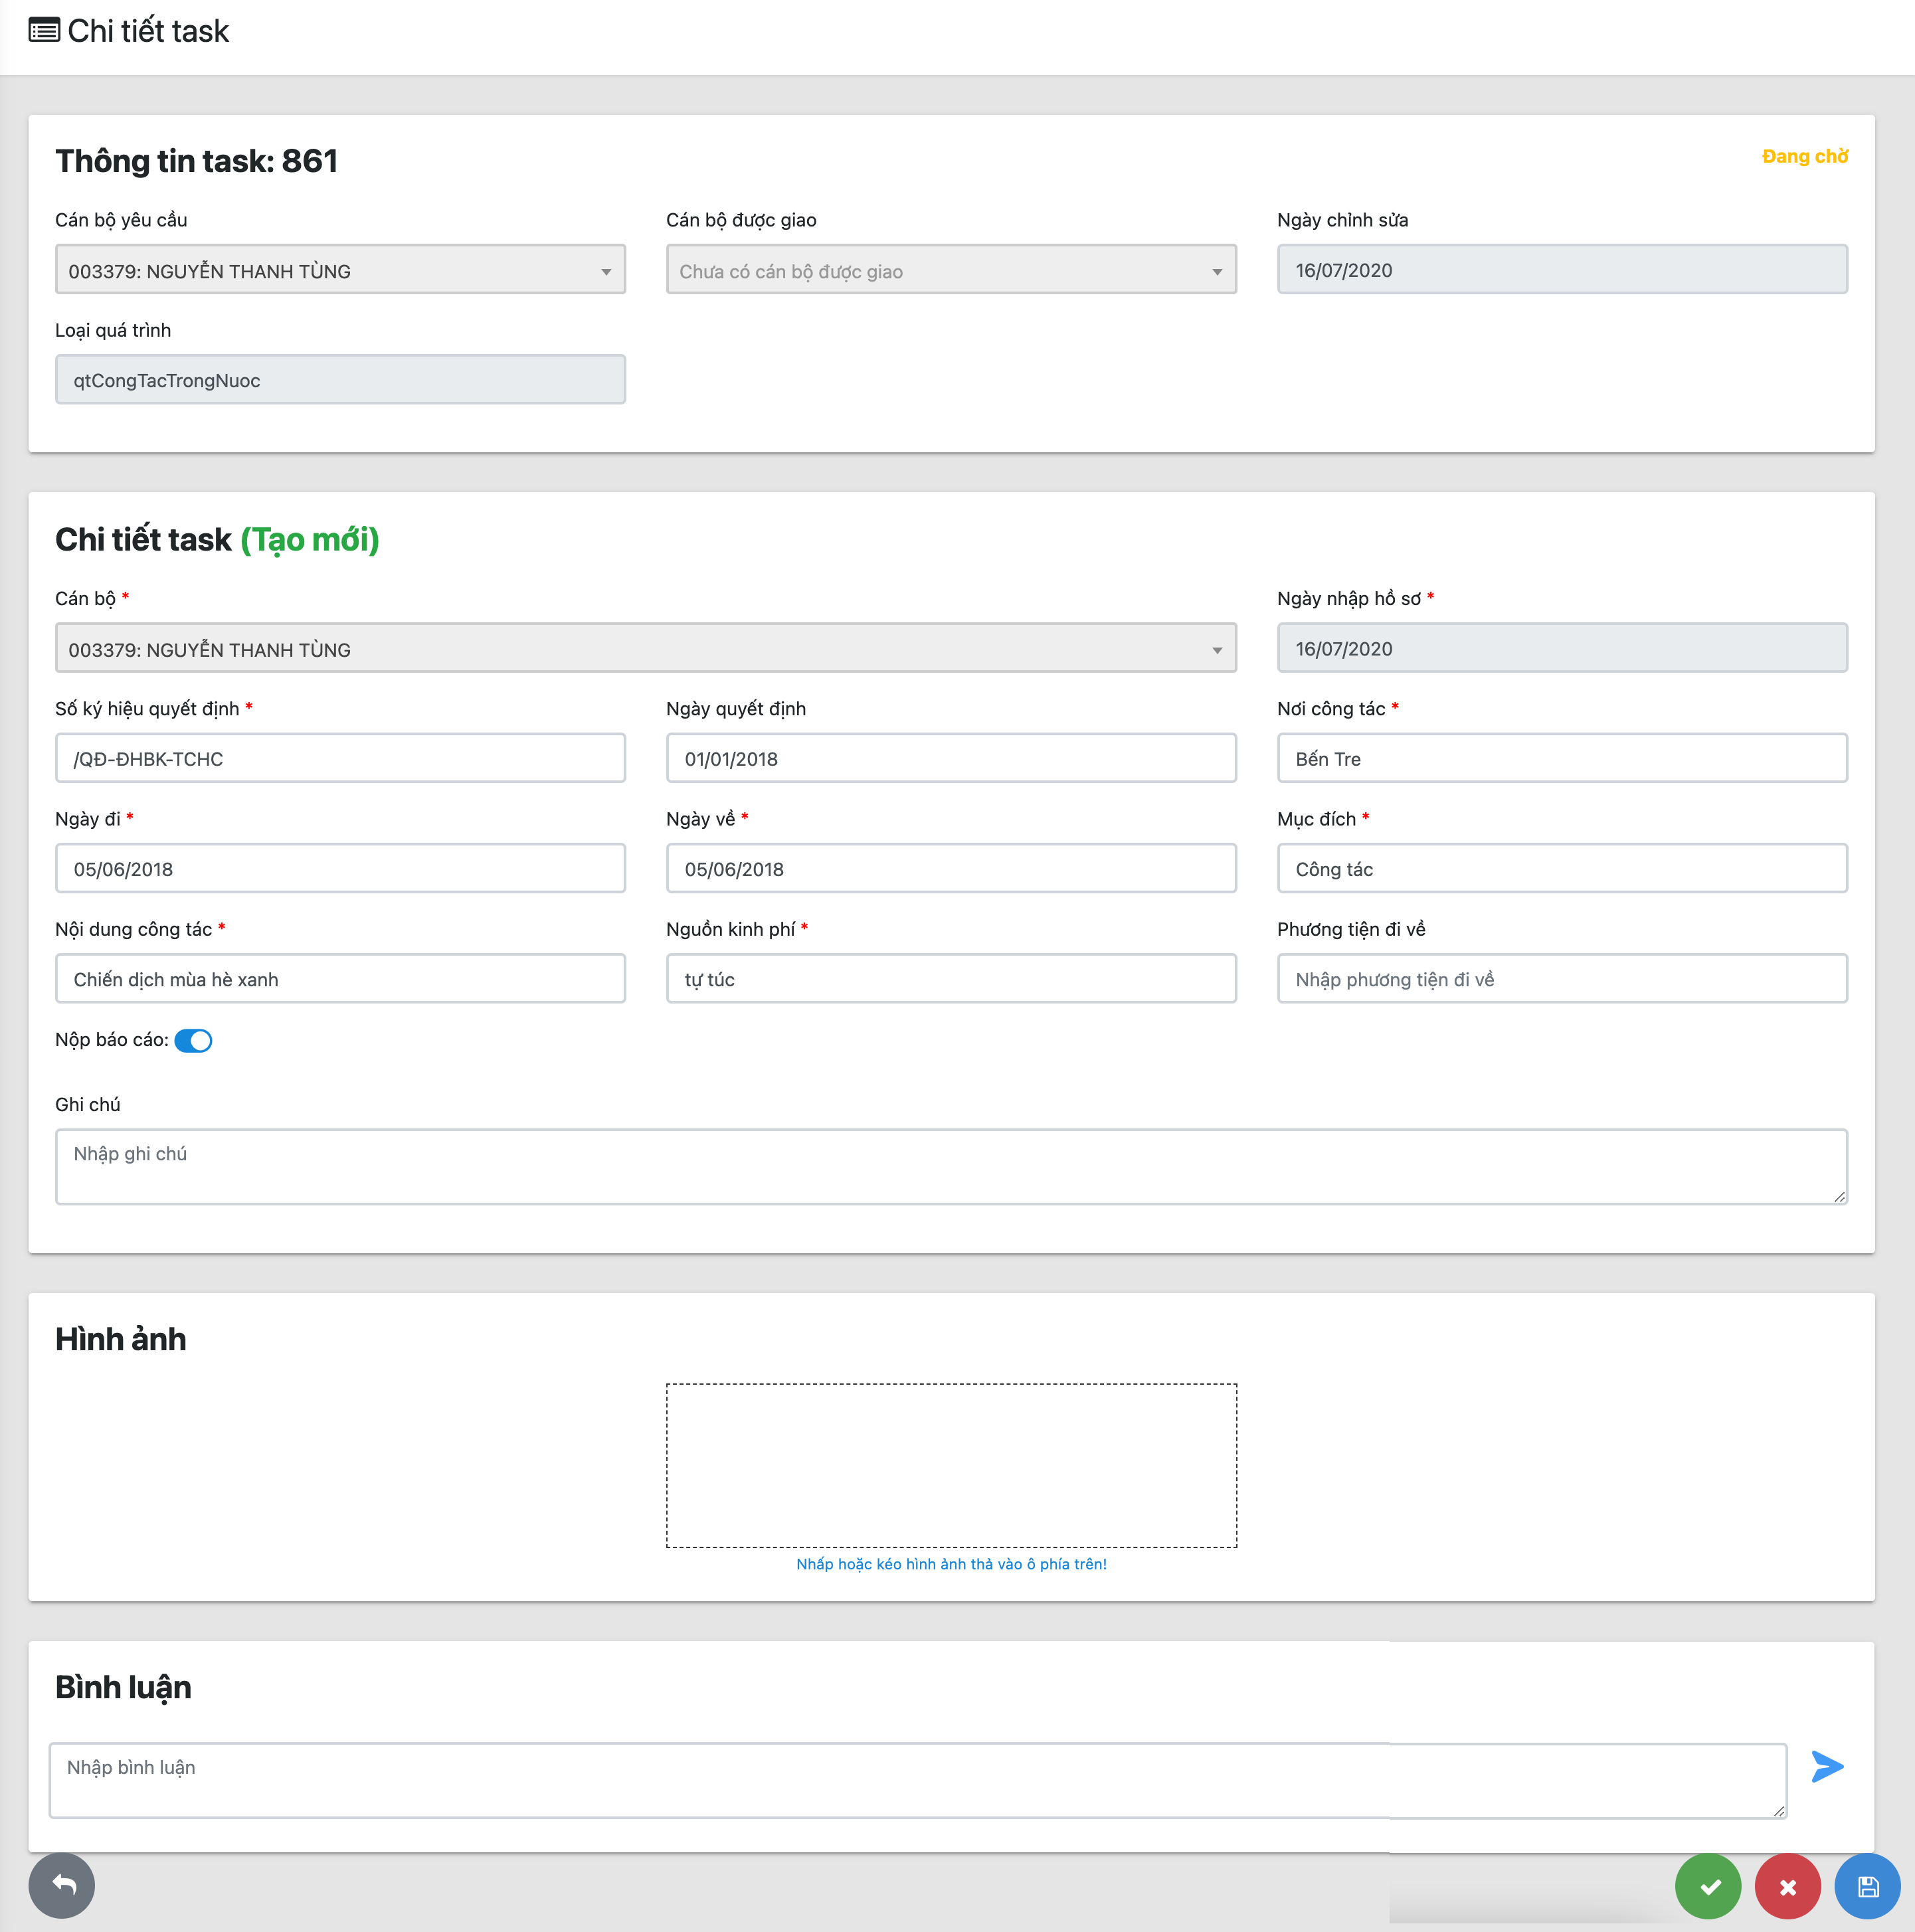
\includegraphics[width=15cm]{img/test/taskDetailAdmin.png}
  \captionof{figure}{Chi tiết yêu cầu}
\end{center}

Duyệt yêu cầu
\begin{center}
  \captionsetup{type=figure}
  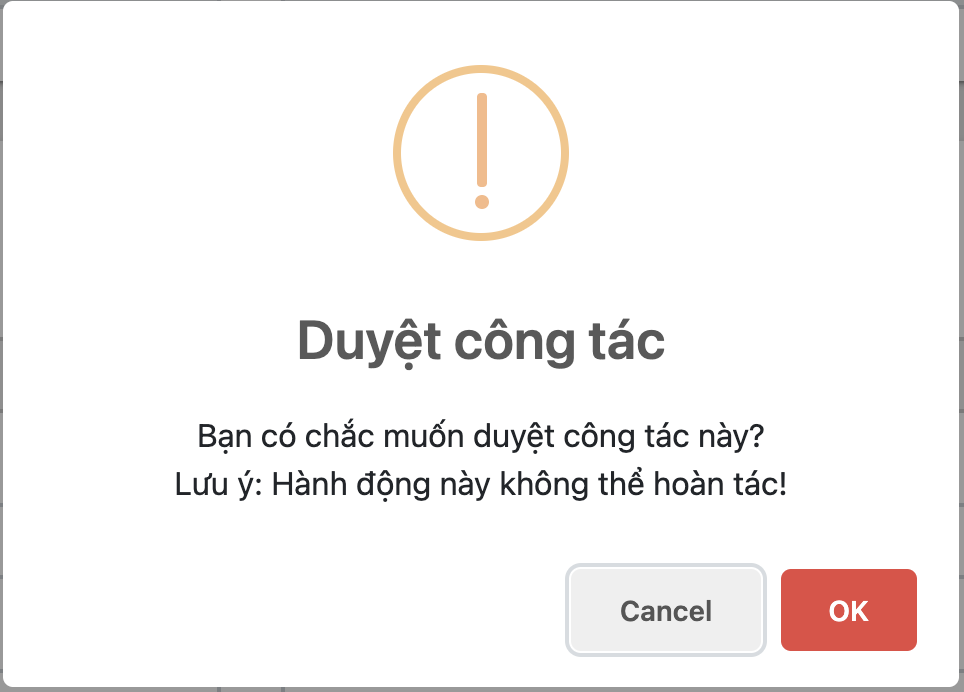
\includegraphics[width=10cm]{img/test/confirmApprove.png}
  \captionof{figure}{Xác nhận duyệt yêu cầu}
\end{center}
Yêu cầu đã được duyệt thành công
\begin{center}
  \captionsetup{type=figure}
  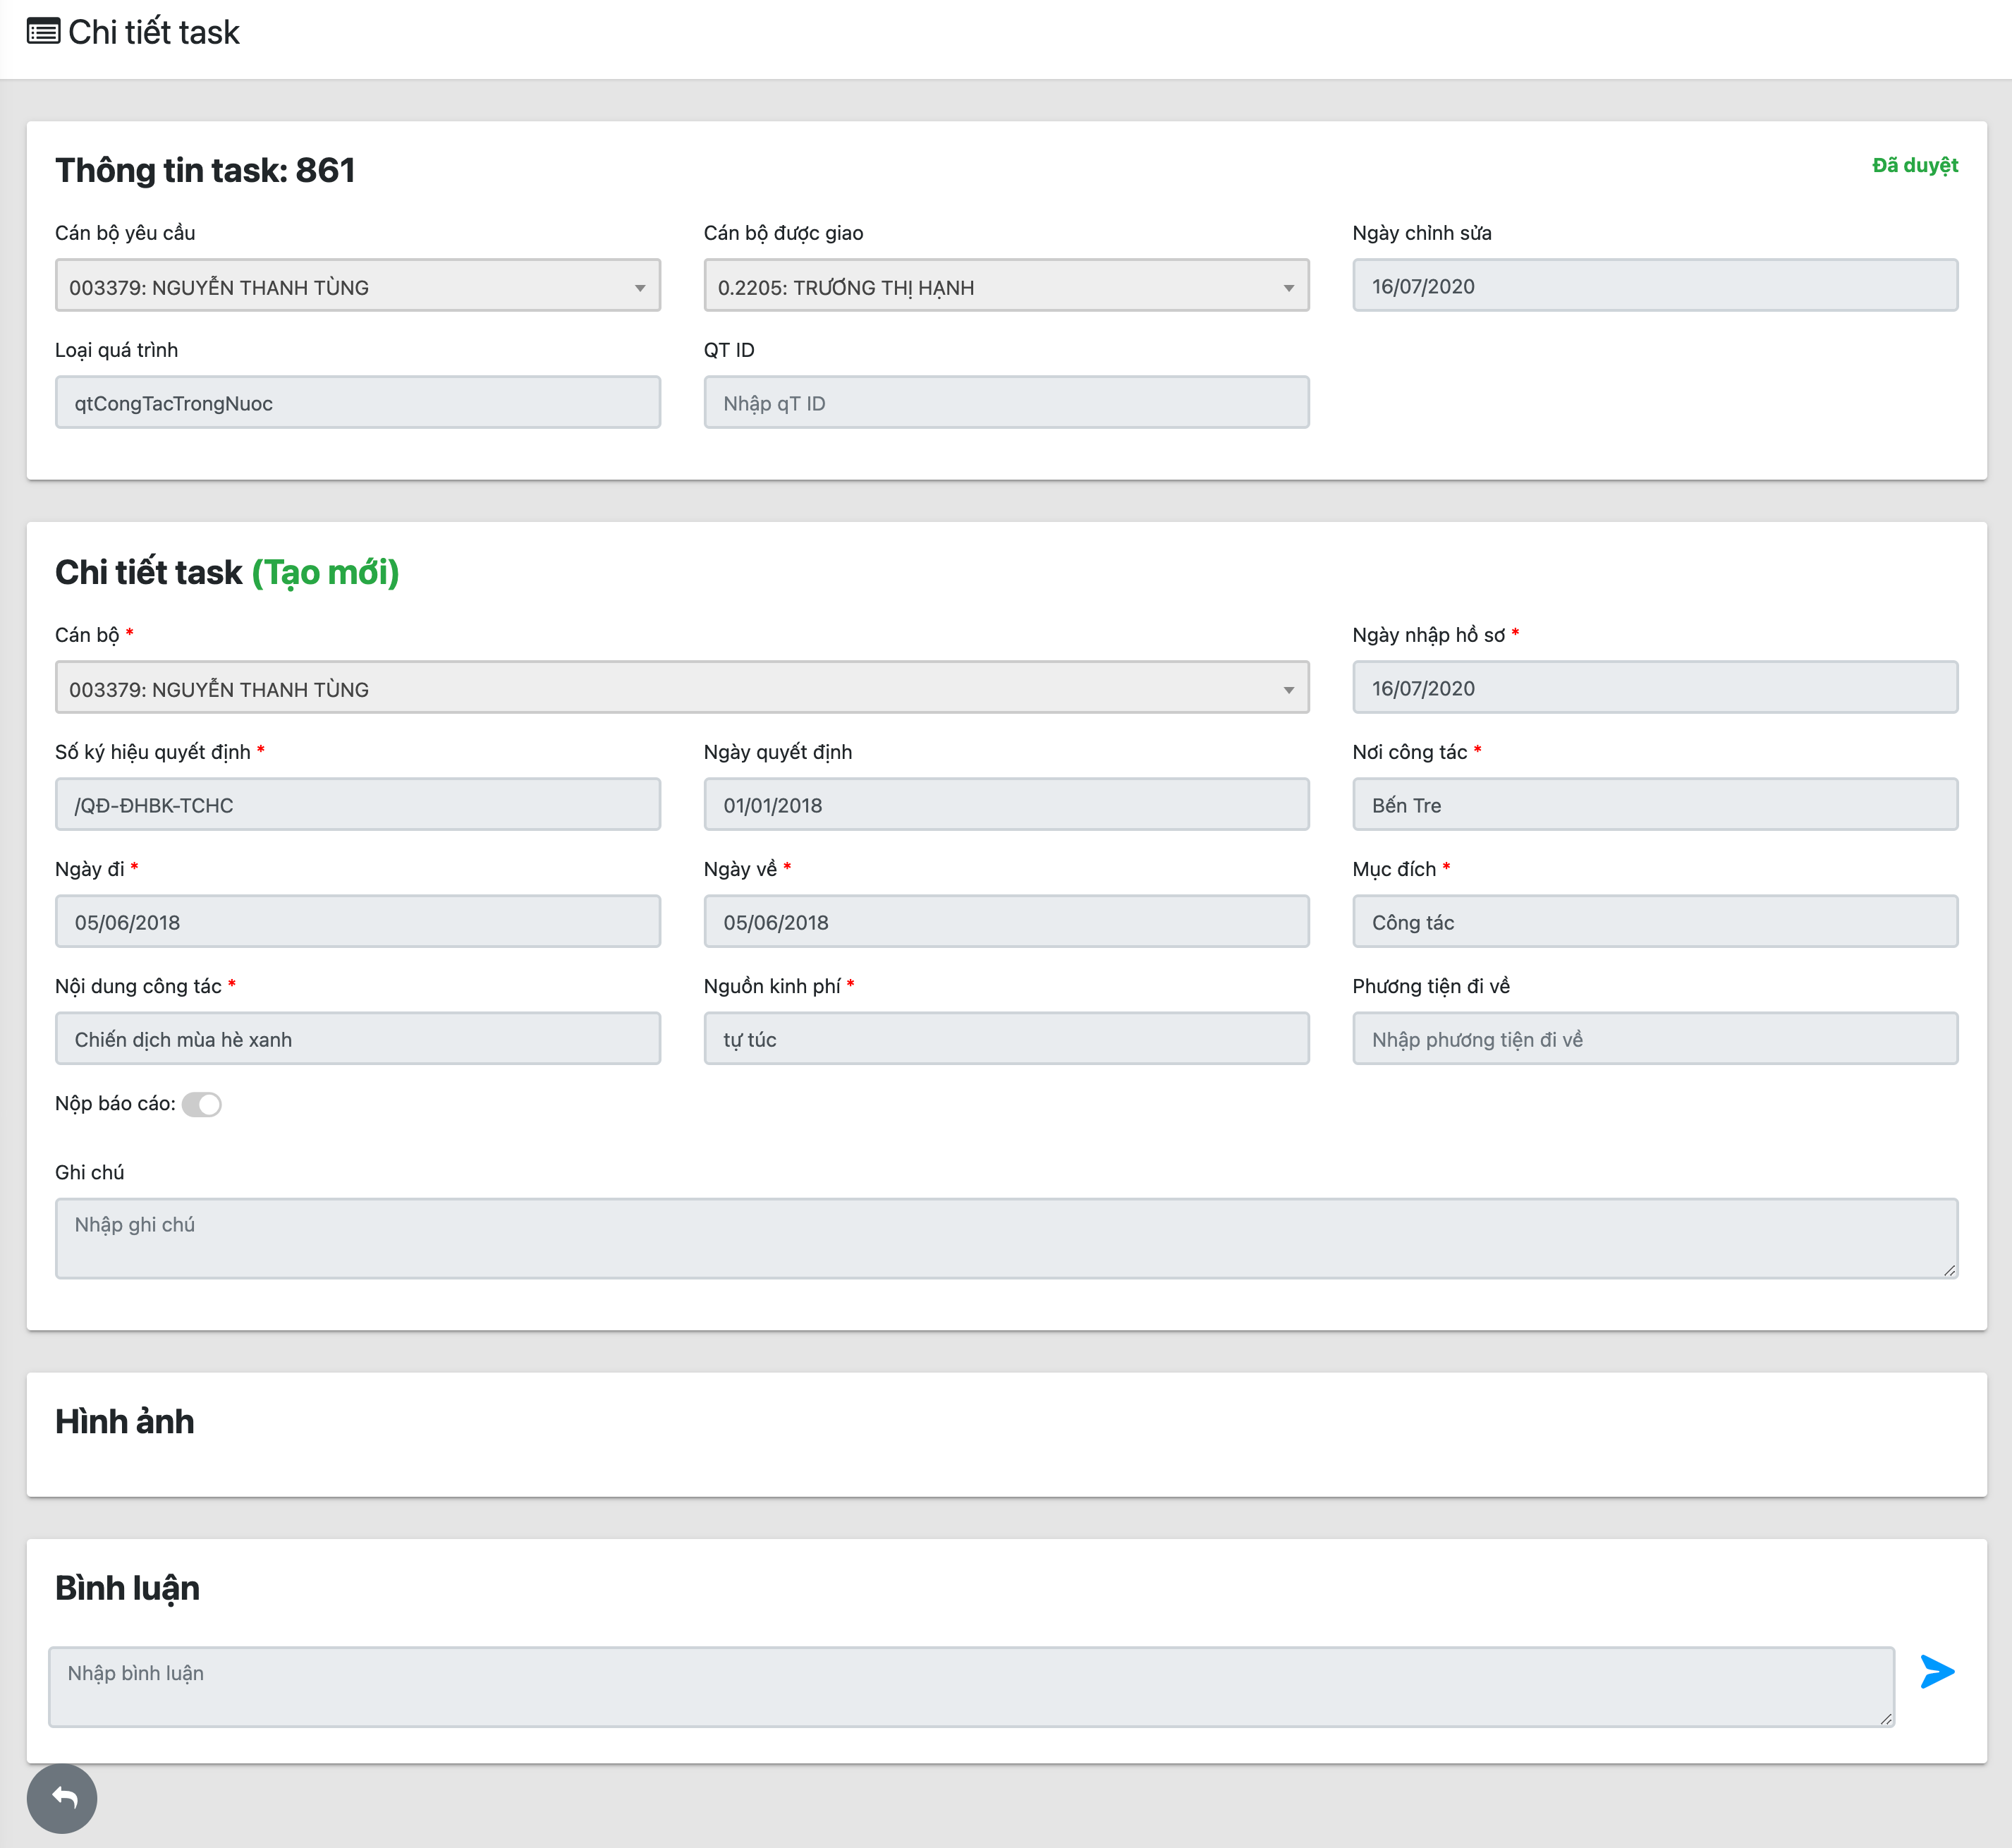
\includegraphics[width=15cm]{img/test/approved.png}
  \captionof{figure}{Duyệt yêu cầu thành công}
\end{center}
Một quá trình công tác trong nước mới đã được thêm vào danh sách quá trình công tác trong nước.
\begin{center}
  \captionsetup{type=figure}
  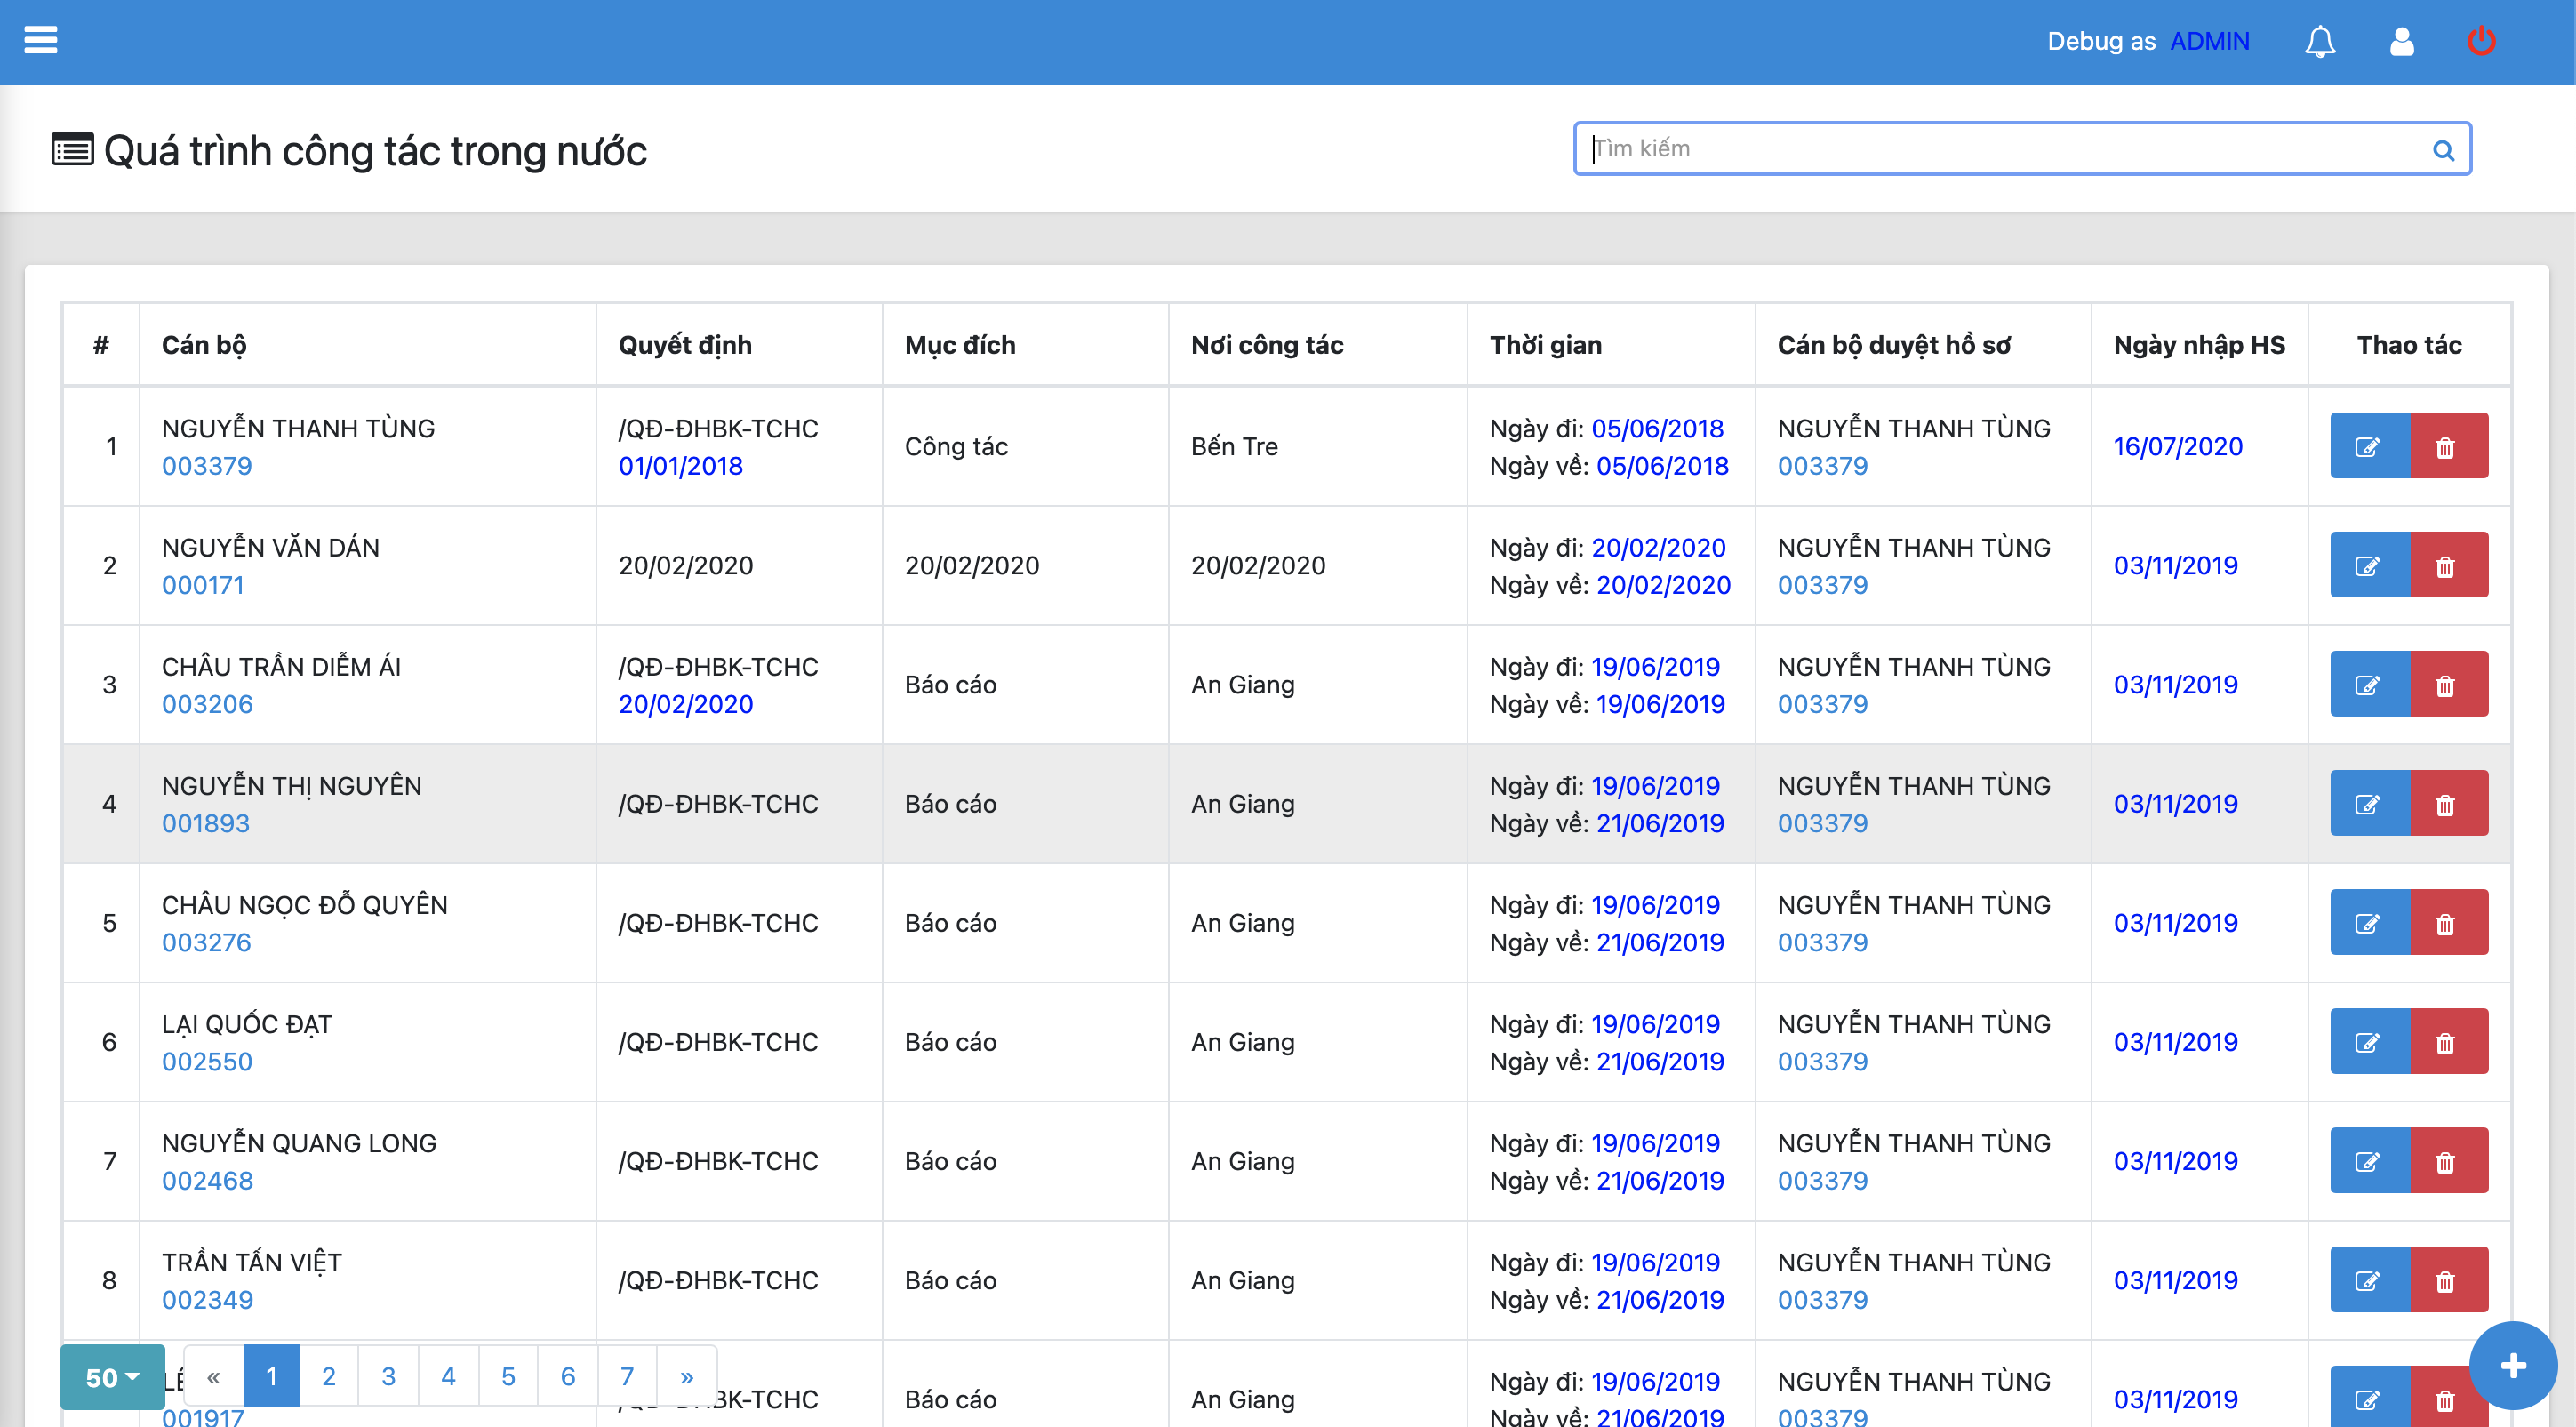
\includegraphics[width=15cm]{img/test/viewLast.png}
  \captionof{figure}{Một quá trình mới được thêm vào danh sách quá trình công tác trong nước}
\end{center}
\section{Kiểm thử chấp nhận (Acceptance Test)}
Kiểm thử chấp nhận là quá trình kiểm thử được thực hiện bởi khách hàng để xác nhận hệ thống có hoạt động đúng như mong đợi với các yêu cầu của khách hàng. Đây là giai đoạn thử nghiệm cuối cùng trước khi hệ thống được đưa vào hoạt động chính thức. 

Hệ thống sẽ được bàn giao với cán bộ phòng Tổ chức-Hành chính để kiểm tra lần cuối trước khi đưa vào sử dụng.